\documentclass[10pt,journal,compsoc]{IEEEtran}

\usepackage{textcomp} % textdegree symbol

%\usepackage{ifpdf}
% Heiko Oberdiek's ifpdf.sty is very useful if you need conditional
% compilation based on whether the output is pdf or dvi.
% usage:
% \ifpdf
%   % pdf code
% \else
%   % dvi code
% \fi

% *** CITATION PACKAGES ***
%
\ifCLASSOPTIONcompsoc
  % IEEE Computer Society needs nocompress option
  % requires cite.sty v4.0 or later (November 2003)
  \usepackage[nocompress]{cite}
\else
  % normal IEEE
  \usepackage{cite}
\fi

% *** GRAPHICS RELATED PACKAGES ***
%
\ifCLASSINFOpdf
  \usepackage[pdftex]{graphicx}
\else
  % \usepackage[dvips]{graphicx}
\fi

% *** MATH PACKAGES ***
\usepackage{amsmath}

% *** SPECIALIZED LIST PACKAGES ***
%\usepackage{algorithmic}

% *** ALIGNMENT PACKAGES ***
%\usepackage{array}

% *** SUBFIGURE PACKAGES ***
%\ifCLASSOPTIONcompsoc
%  \usepackage[caption=false,font=footnotesize,labelfont=sf,textfont=sf]{subfig}
%\else
%  \usepackage[caption=false,font=footnotesize]{subfig}
%\fi

% *** FLOAT PACKAGES ***
% \usepackage{float}
% \usepackage{fixltx2e}
% \usepackage{stfloats}
% \usepackage{dblfloatfix}

%\ifCLASSOPTIONcaptionsoff
%  \usepackage[nomarkers]{endfloat}
% \let\MYoriglatexcaption\caption
% \renewcommand{\caption}[2][\relax]{\MYoriglatexcaption[#2]{#2}}
%\fi

% *** PDF, URL AND HYPERLINK PACKAGES ***
\usepackage{url}


% An example of a floating figure using the graphicx package.
% Note that \label must occur AFTER (or within) \caption.
% For figures, \caption should occur after the \includegraphics.
% Note that IEEEtran v1.7 and later has special internal code that
% is designed to preserve the operation of \label within \caption
% even when the captionsoff option is in effect. However, because
% of issues like this, it may be the safest practice to put all your
% \label just after \caption rather than within \caption{}.
%
%\begin{figure}[!t]
%\centering
%\includegraphics[width=2.5in]{myfigure}
% where an .eps filename suffix will be assumed under latex,
% and a .pdf suffix will be assumed for pdflatex; or what has been declared
% via \DeclareGraphicsExtensions.
%\caption{Simulation results for the network.}
%\label{fig_sim}
%\end{figure}

% Note that the IEEE typically puts floats only at the top, even when this
% results in a large percentage of a column being occupied by floats.


% An example of a double column floating figure using two subfigures.
% (The subfig.sty package must be loaded for this to work.)
% The subfigure \label commands are set within each subfloat command,
% and the \label for the overall figure must come after \caption.
% \hfil is used as a separator to get equal spacing.
% Watch out that the combined width of all the subfigures on a
% line do not exceed the text width or a line break will occur.
%
%\begin{figure*}[!t]
%\centering
%\subfloat[Case I]{\includegraphics[width=2.5in]{box}%
%\label{fig_first_case}}
%\hfil
%\subfloat[Case II]{\includegraphics[width=2.5in]{box}%
%\label{fig_second_case}}
%\caption{Simulation results for the network.}
%\label{fig_sim}
%\end{figure*}
%
% Note that often IEEE papers with subfigures do not employ subfigure
% captions (using the optional argument to \subfloat[]), but instead will
% reference/describe all of them (a), (b), etc., within the main caption.
% Be aware that for subfig.sty to generate the (a), (b), etc., subfigure
% labels, the optional argument to \subfloat must be present. If a
% subcaption is not desired, just leave its contents blank,
% e.g., \subfloat[].


% An example of a floating table. Note that, for IEEE style tables, the
% \caption command should come BEFORE the table and, given that table
% captions serve much like titles, are usually capitalized except for words
% such as a, an, and, as, at, but, by, for, in, nor, of, on, or, the, to
% and up, which are usually not capitalized unless they are the first or
% last word of the caption. Table text will default to \footnotesize as
% the IEEE normally uses this smaller font for tables.
% The \label must come after \caption as always.
%
%\begin{table}[!t]
%% increase table row spacing, adjust to taste
%\renewcommand{\arraystretch}{1.3}
% if using array.sty, it might be a good idea to tweak the value of
% \extrarowheight as needed to properly center the text within the cells
%\caption{An Example of a Table}
%\label{table_example}
%\centering
%% Some packages, such as MDW tools, offer better commands for making tables
%% than the plain LaTeX2e tabular which is used here.
%\begin{tabular}{|c||c|}
%\hline
%One & Two\\
%\hline
%Three & Four\\
%\hline
%\end{tabular}
%\end{table}

% correct bad hyphenation here
\hyphenation{multi-modal inter-cultural net-works }


\begin{document}

\title{Laughing and engagement in spontaneous~interactions:
       analysis of Estonian and North~Sami conversational data}

\author{Kristiina~Jokinen, Katri~Hiovain, Trung Ngo Trong,
        and~Graham~Wilcock% <-this % stops a space
\IEEEcompsocitemizethanks{\IEEEcompsocthanksitem K. Jokinen is with the Institute of Behavioural Sciences, University of Helsinki, Helsinki, Finland.\protect\\
% note need leading \protect in front of \\ to get a newline within \thanks as
% \\ is fragile and will error, could use \hfil\break instead.
E-mail: kristiina.jokinen@helsinki.fi
\IEEEcompsocthanksitem J. Doe and J. Doe are with Anonymous University.}% <-this % stops an unwanted space
\thanks{Manuscript received April 19, 2005; revised August 26, 2015.}}

% The paper headers
\markboth{Journal of \LaTeX\ Class Files,~Vol.~14, No.~8, August~2015}%
{Shell \MakeLowercase{\textit{et al.}}: Bare Demo of IEEEtran.cls for Computer Society Journals}
% *** Note that you probably will NOT want to include the author's ***
% *** name in the headers of peer review papers.                   ***
% You can use \ifCLASSOPTIONpeerreview for conditional compilation here if
% you desire.

% for Computer Society papers, we must declare the abstract and index terms
% PRIOR to the title within the \IEEEtitleabstractindextext IEEEtran
% command as these need to go into the title area created by \maketitle.
% As a general rule, do not put math, special symbols or citations
% in the abstract or keywords.
\IEEEtitleabstractindextext{%
\begin{abstract}
This article focuses on laughter types in Estonian and North Sami conversations, and in particular, studying the types of laughter in their multimodal context (head movement). The questions that we aim to answer are:
(1) What kind of differences are there in terms of acoustic features between the different types of laughters?
(2) Are the different types of laughter distributed similarly among the conversation partners?
(3) Do the partners share laughter equally or does one type get shared more often?
(4) Do the different types show different levels of engagement among the partners?
We first study acoustic properties of laughter types and then employ deep learning techniques to analyse the corpus in regard to laughter signal recognition. The multimodal analysis used simple visual features from the bounding boxes that describe the person's head movement in the video.
Our results confirm the hypothesis of the synchrony of body movements with laughter, but we also acknowledge the complexity of the problem and the need for further investigations on the feature sets and the algorithm used.
\end{abstract}
}
% Note that keywords are not normally used for peerreview papers.
%\begin{IEEEkeywords}
%Computer Society, IEEE, IEEEtran, journal, \LaTeX, paper, template.
%\end{IEEEkeywords}}

% make the title area
\maketitle


\IEEEdisplaynontitleabstractindextext

% For peer review papers, you can put extra information on the cover
% page as needed:
% \ifCLASSOPTIONpeerreview
% \begin{center} \bfseries EDICS Category: 3-BBND \end{center}
% \fi
%
% For peerreview papers, this IEEEtran command inserts a page break and
% creates the second title. It will be ignored for other modes.
\IEEEpeerreviewmaketitle



\IEEEraisesectionheading{\section{Introduction}\label{sec:introduction}}

In this paper, we focus on laughter and speech-laugh in Estonian and North Sami conversations, and in particular, studying the types of laughter in their multimodal context (facial and head movement). The data consists of two data sets which differ in that the Estonian conversations are first-encounter dialogues where the participants do not know each other in advance and make acquaintance with each other, and the North Sami dialogues are among people who know each other: group of friends and school mates or teacher-student conversations. The two languages are linguistically related but represent culturally very different communities.

Laughter is commonly related to joking and amusement, and it has been studied in humour studies \cite{Chafe:07}. However, laughter does not occur in humorous contexts only, but in potentially face-threatening situations where it is a sign of politeness and socially acceptable behaviour. In sociolinguistic research, laughter is regarded as a typical social phenomenon, described as serving a broad range of interactional functions. Goffman \cite{Goffman:74} talks about situated interactions and the bursts of laughter that break the ordinary interactional frames. In a seminal work on the organization of laughter in talk with the Conversation Analysis, Jefferson \cite{Jefferson:84} focussed on interactional consequences of laughter, and pointed out that the partner may choose to be silent in which case laughing and silence are two systematic possibilities for joke completions. Speech research has focussed on the acoustic analysis of laughter and on the categorization of various forms of laughter for the purposes of emotion recognition or speech synthesizer (\cite{Trouvain:03}, \cite{Truong:vanLeeuwen:07}, \cite{Owren:Bachorowski:07}, \cite{Bachorowski:ea:01}, \cite{Tanaka:Campbell:11}).

Acoustic properties of laughter vary a lot between speakers and within a speaker, but it is generally concluded that F0 formant is much higher in laughter than in speech, and that the ratio of the length of unvoiced to voiced parts is greater for laughter than for speech (\cite{Bachorowski:ea:01}, \cite{Truong:vanLeeuwen:07}).

Classifications of laughter often distinguish between free-laughter and speech-laugh, i.e. laughter which is synchronous with speech. Nwokah et al. \cite{Nwokah:ea:99} found that up to 50\% of laughs overlap with speech in their corpus of mother and child communication, and also that the duration of speech-laugh was significantly longer than that of only laughter (1.24s vs. 1.07s). Often laughs are divided into polite and amused smiles, and e.g. Hoque et al. \cite{Hoque:ea:11} found that polite smiles are more likely to be socially conditioned, masking and controlled smiles, while the amused ones are more likely to be genuine. Tanaka and Campbell \cite{Tanaka:Campbell:11} used a four-way classification, with the most common distinction between the spontaneous mirthful laugh and polite laugh, which together apparently account for 80\% of the laughs. In recent studies on social and situational signals and their correlation with the interactional context (\cite{Bonin:ea:14}, \cite{Bonin:16}) it is shown that when laughter functions as a social signal, its timing is structured and conveys information about the underlying discourse structure. Higher amounts of laughter occur in topic transition moments than in topic continuation moments and when the temporal distance from the topic boundary increases, laughter becomes more likely to occur. Gilmartin et al. \cite{Gilmartin:ea:13} studied laughter and engagement and noted that a significant change in the amount of laughter occurs at fifteen seconds around the topic changes.

\section{Research Questions}
\label{sec:research-questions}

Laughter is usually related to joking and humour, but it also occurs in connection to socially critical situations such as signalling relief of embarrassment. We assume that laughing is, first of all, a means of creating common understanding and rapport among the participants, i.e. an effective feedback signal that the participants use to show benevolent contact and their willingness to continue the interaction. However, we also hypothesize that laughing used as an interaction strategy to distance oneself from the partner and from the discussed topics, i.e. it is an acceptable way to disassociate oneself from the conversation.

Our main research questions in this study concern understanding the conversational participants' laughter behaviour when they interact with each other in non-scripted friendly conversations. When people exhibit laugher or speech-laugh (speak in a laughing tone):

\begin{enumerate}
\item What kind of differences are there in terms of acoustic features (F0, intensity, duration) between the different types of laughters?
\item Are the different types of laughter distributed similarly among the conversation partners?
\item Do the partners share laughter equally or does one type get shared more often?
\item Do the different types show different levels of engagement among to partners?
\end{enumerate}

These questions are important in the context of human communication studies so as to gain a deeper understanding of the functions and role of laughter in human face-to-face conversations. The insights on these questions can help develop models for intelligent agents (e.g. robot agents or virtual agents) that allow the agent to recognize and understand human laughter behaviour, and then appropriately react to this. Moreover, we can also motivate the research by models that allow the agent to mimic face-to-face interactions with other humans so as to provide more natural interaction that facilitates creation of rapport and mutual bonds.
An important aspect also deals with intercultural comparisons related to the participants' engagement and synchrony in various communicative activities, and building models for their automatic processing. However, the corpora we have used in the acoustic and multimodal analyses are rather small and varied in order to warrant reliable cultural comparisons. Such work is left for later research.

The paper is structured as follows.
We first introduce the two corpora in Section~\ref{sec:corpora-annotations}:
the Estonian MINT corpus and the North Sami DigiSami corpus.
We then define the different laughter types in Section~\ref{sec:laughter-types},
and provide discussion and comparison of the laughter statistics from the two corpora
in Section~\ref{sec:statistics}.
We present the results of our acoustic analysis in Section~\ref{sec:acoustic-analysis}
and the results of our deep-learning analysis in Section~\ref{sec:automatic-laughter-detection}.
We provide further discussion and point to future research directions in Section~\ref{sec:discussion},
and conclude in Section~\ref{sec:conclusion}.

\begin{table*}[!t]
\caption{The Annotated Laughter Types}
\label{tab:laughter-types}
\centering
\begin{tabular}{| p{0.2cm} | p{1.7cm} | p{12cm} |}
\hline
fl	& free-laughter	& laughter without speaking simultaneously \\ \hline
st	& speech-laugh	& laughter and speech combined \\ \hline
b	& breath	    & heavy breathing, smirk, sniff; unvoiced, glottal sounds and sibilants \\ \hline
e	& embarrassed	& speaker is embarrassed, confused, uncertain; disassociating  \\ \hline
m	& mirth	        & fun, humorous, real laughter, occurring when telling jokes etc. \\ \hline
d	& derision	    & mocking the partner \\ \hline
p	& polite	    & polite laughter showing positive attitude towards the other speaker \\ \hline
o	& other    	    & laughter that doesn't fit in the previous categories; acoustically unusual laughter\\ \hline
\end{tabular}
\end{table*}

\begin{table*}[!t]
\caption{Laughter Types in the DigiSami Corpus}
\label{tab:laughter-digisami}
\centering
\begin{tabular}{| l | r | r r | r r r r r r | r | r |}
\hline
Conversation & Duration & fl  & st & m & b & e & d & p & o & Total & per minute \\
\hline
02\_V  & 13:33 & 138 & 36 & 28 & 87 & 59 & 0 & 0 & 0 & 174 & 13.14 \\
06\_PS & 11:44 &   0 & 10 &  4 &  4 &  0 & 0 & 2 & 0 &  10 &  8.70 \\
05\_TP &  8:33 &  18 & 37 & 27 & 27 &  0 & 0 & 0 & 1 &  55 &  6.60 \\
08\_VV & 12:29 &  12 & 22 & 19 & 15	&  0 & 0 & 0 & 0 &  34 &  2.76 \\
01\_S  & 16:29 &  25 & 18 & 14 & 20 &  6 & 2 & 0 & 1 &  43 &  2.64 \\
04\_S  &  3:28 &   3 &  4 &  2 &  3 &  1 & 0 & 0 & 1 &   7 &  2.16 \\
03\_V  &  8:02 &   2 & 12 &  6 &  8 &  0 & 0 & 0 & 0 &  14 &  1.74 \\
07\_SX &  6:44 &   0 &  4 &  0 &  2	&  0 & 0 & 2 & 0 &   4 &  0.60 \\
\hline
Total  & Mean  & 198 & 143 & 100 & 166 & 66 & 2 & 4 & 3 & 341 & \\
\%     & 10:07 &  58 &  42 &  29 &  49 & 19 & & 3 &	& 100 & \\
\hline
\end{tabular}
\end{table*}

%%%%%%%%%%%%%%%%%%%%%%%%%%%%%%%%%%%%%%%%%%%%%%%%%%%%%%%%%%%%%%%%%%%%%%
%%% Section 3
\section{The Corpora and their Annotations}
\label{sec:corpora-annotations}

\subsection{The North Sami DigiSami Corpus}
\label{sec:digisami-corpus}

The DigiSami Corpus of spoken North Sami was collected in the areas traditionally inhabited by the Sami people: in Enonteki\"{o}, Utsjoki, Inari and Ivalo in Finland, and in Kautokeino and Karasjok in Norway.
%(see the map in Figure~\ref{fig:data-locations}).
North Sami belongs to the Fenno-Ugric language family, and is one of the Sami languages
spoken in Northern Scandinavia, Finland and the Kola Peninsula \cite{Hirvonen:ea:97}.
%\cite{Seurujarvi-Kari:ea:97}.
All the speakers are native speakers of North Sami, and their ages vary between 16 and 65 years.
The data is thus versatile, including informants from two different countries and of different ages.
More details about the data collection can be found in \cite{Jokinen:Wilcock:SLTU:14} and \cite{Jokinen:LREC:14}).

The participants were invited to take part in three different tasks: discussion and writing Wikipedia articles, reading aloud of existing Wikipedia texts, and taking part in a free conversation which was video recorded. However, in the context of studying laughing and engagement, only the conversations are considered.
The conversations were recorded by EDIROL R4Pro four-channel recording device with AKG 417 L-microphones. Two Panasonic HC-X920 video cameras and three GoPro HERO3 cameras were used for video-recordings. Conversational speech was also recorded by the cameras own microphone. The conversations were between two or three people, and the participants were instructed to discuss freely about their own interests or about the Wikipedia articles they were to write (e.g. Sami language, Sami costume, music, reindeer herding, and snow-mobiles). The topics vary from everyday life (next vacation, driving school, cars) to translation between Sami and other languages and to technological tools that have been made to help writing North Sami more correctly. The conversations differ in style: familiar participants have casual conversations and they often refer to things they had been talking about earlier. The conversations between a pupil and a teacher are fairly formal, and the topics stick to the forthcoming task, i.e. things that one could write a Wikipedia article about.

The corpus consists of more than three hours (195 minutes) of annotated data; the mean duration of the conversations was 10:07 minutes, and it is valuable because it is the first North Sami conversational corpus. The total number of laughter occurrences in the North Sami data is 341 in 8 different conversations. Two of these conversations were recorded in Karasjok, Norway, and the rest in Ivalo and Utsjoki, Finland. There were 19 conversation informants altogether. 11 of the participants were female and 8 were male. Altogether, 59\% (201) of the laughter occurrences were performed by a female informant, while 41\% (140) were performed by a male informant. Table~\ref{tab:laughter-digisami} shows the number of different laughter types in different conversations.

\subsection{The Estonian MINT Corpus}
\label{sec:estonian-mint-corpus}

The Estonian First Encounters data was collected in the project MINT \cite{Jokinen:Tenjes:12}. The MINT corpus of first encounters follows the guidelines of the project NOMCO \cite{Paggio:ea:10}. The first encounter dialogues engage participants, who do not know each other in advance, in an activity where their task is to chat and make acquaintance with each other. Original data was collected in the Estonian language, and the data is annotated and analysed using an annotation scheme which is co-measurable with the annotations used in NOMCO. Each participant was given a short presentation of the project and the goals of the data collection before the recording, and they were also asked to sign a consent form (in the Estonian language) that grants permission for their video data to be used for research purposes, and to be shown to third parties without further permission.

SonyHDR-XR550V cameras with three external Sony ECM-HW2 wireless microphones were used in the recordings. The microphones were paired with cameras so that each camera had its own audio track. The video recording was on the full HD quality mode, and the camera views were cut, edit and merged via Sony Vegas Pro 11.
% See Figure 2.

There were a total of 23 participants (12 male and 11 female), with age ranging between 21 and 61 years. The participants are native speakers of Estonian and they are students or university employees. All conversations were two-participant dialogues, and each participant had two conversations with two different partners. The interactions were gender balanced so that there were 8 female-female encounters, 7 female-male encounters, and 8 male-male encounters. The corpus contains 23 conversations, and the mean duration of the interaction was 5:52 minutes.

None of the participants knew each other beforehand, as opposed to the DigiSami data, in which all participants knew each other or were even close friends. In most conversations, the topics were related to introductory and self-presentation issues, mainly studies or work.

The laughter occurrences in the Estonian MINT Corpus were annotated as described in Table~\ref{tab:laughter-types}. The total number of laughter occurrences in the Estonian MINT data was 519 in 23 different conversations.
%All conversations had 2 participants and the mean duration of the conversations was 5:52 minutes. 22 of the participants were female and 24 male - each participant attended 2 different conversations with a different partner (one participant had 2 different partners).
Altogether, 67\% (348) of the laughter occurrences were performed by a female informant, while 33\% (171) were performed by a male informant.

\subsection{The Finnish NOMCO Corpus}
\label{sec:finnish-nomco-corpus}
The research material consists of the Finnish first encounters dialogue corpus collected as part of the NOMCO project, a Nordic cooperation project. The project aim for developing and analyzing multi-modal spoken language corpora in the Nordic countries, and to compare communication strategies in three closely related languages (Danish, Finnish, and Swedish).

The interactions in the Finnish first encounters corpora involve two subjects who are standing in front of a light background. The participants were instructed to get to know each other in a short interaction, as they might do at a party or a reception. After the recording they answered a questionnaire about their reactions to both the interlocutor and the interaction setting. The dataset consist of 16 video recordings of first-encounter interactions in Finnish. Video recordings show both participants at the same time as well as each participant individually, and there is also a mosaic version with the individual and the joint video streamed together in one video. In this study we concentrate on individual behaviours and not on interpersonal communication, and thus used the individual videos rather than videos with both participants as research material.

There are 14 participants - 4 males and 10 females, whom did not know each other in advance. All participants are native speakers of Finnish. Of the 16 collected conversations, there are 2 male-male conversations, 6 male-female conversations, and 8 female-female conversations. The shortest conversation is 3 minutes 49 seconds and the longest 8 minutes 2 seconds. The average length of the conversations is 6 minutes 25 seconds. Eleven of the participants had two conversations with a different partner, while three took part in only one conversation. Although one’s conversational activity depends on the partner, it seems useful to distinguish between the first and the second conversation, since in the second one, the speaker is familiar with the recording situation and can therefore feel more relaxed and attentive to the partner. In fact, in terms of the speaking time, the participants seem to speak about 7\% more in their first conversation than in the second one, which can be interpreted as supporting this assumption: in the second conversation, they feel more experienced and in control of the situation, so as to follow and let the partner to speak.

\textbf{TODO}: Add more statistics of Finnish laughter.

\section{Laughter Types}
\label{sec:laughter-types}

For the purposes of measuring engagement and to understand how laughing functions as part of conversations, we annotated the data with laughter features using Praat. Following the previous research, the laughter annotation included the markers for the two laughter types free-laugh (fl) and speech-laugh (st), and for the more specific characterization: 'm' - mirth, 'e' - embarrassed, 'b' - breath, 'p' - polite, 'd' - derision and 'o' - other. Table~\ref{tab:laughter-types} presents the laughter types with explanations.

\begin{table*}[!t]
\caption{Laughter Types in the Estonian MINT Corpus}
\label{tab:laughter-estonian}
\centering
\begin{tabular}{| l | r | r r | r r r r r | r | r |}
\hline
Conversation & Duration & fl  & st & m & b & e & p & o & Total & per minute \\
%Conv. & Dur. & fl  & st & m & b & e & p & o & Tot. \\
\hline
C\_1 & 5:50 & 18 & 13 & 10 & 14 & 7 & 0 & 0 & 31 & 5.64 \\
C\_2 & 6:19 &  9 & 13 &  9 & 10 & 0 & 3 & 0 & 22 & 3.55 \\
C\_3 & 6:08 & 12 &  4 &  7 &  8 & 0 & 1 & 0 & 16 & 2.63 \\
C\_4 & 6:20 & 17 &  3 &  0 & 12 & 3 & 5 & 0 & 20 & 3.23 \\
C\_5 & 6:33 & 26 & 15 & 16 & 15 & 7 & 3 & 0 & 41 & 6.48 \\
C\_6 & 6:18 & 18 & 22 & 27 & 11 & 2 & 0 & 0 & 40 & 6.47 \\
C\_7 & 6:46 & 11 & 21 &  8 & 24 & 0 & 0 & 0 & 32 & 4.95 \\
C\_8 & 6:49 &  9 &  9 &  8 &  6 & 3 & 1 & 0 & 18 & 2.77 \\
C\_9 & 6:51 & 15 &  7 &  8 & 13 & 0 & 1 & 0 & 22 & 3.38 \\
C\_10 & 5:04 & 4 & 13 &  4 & 13 & 0 & 0 & 0 & 17 & 3.37 \\
C\_11 & 5:42 & 19 & 18 & 23 & 13 & 0 & 1 & 0 & 37 & 6.83 \\
C\_12 & 5:44 & 11 & 11 & 12 &  9 & 1 & 0 & 0 & 22 & 4.04 \\
C\_13 & 6:51 &  2 &  2 &  2 &  2 & 0 & 0 & 0 &  4 & 0.61 \\
C\_14 & 6:07 & 11 &  7 &  3 & 15 & 0 & 0 & 0 & 18 & 2.97 \\
C\_15 & 5:52 &  5 &  2 &  1 &  6 & 0 & 0 & 0 &  7 & 1.27 \\
C\_16 & 5:28 &  4 &  3 &  1 &  6 & 0 & 0 & 0 &  7 & 3.07 \\
C\_17 & 5:18 & 13 & 11 & 12 & 12 & 0 & 0 & 0 & 24 & 4.63 \\
C\_18 & 4:43 & 23 & 15 & 15 & 22 & 0 & 1 & 0 & 38 & 8.58 \\
C\_19 & 5:24 & 14 & 14 &  5 & 20 & 0 & 3 & 0 & 28 & 5.34 \\
C\_20 & 5:01 & 11 &  6 &  2 & 11 & 0 & 0 & 4 & 17 & 3.39 \\
C\_21 & 5:12 &  7 &  3 &  8 &  1 & 0 & 1 & 0 & 10 & 1.95 \\
C\_22 & 5:38 & 17 &  7 &  4 & 19 & 0 & 1 & 0 & 24 & 4.46 \\
C\_23 & 5:08 & 19 &  5 &  4 & 20 & 0 & 0 & 0 & 24 & 4.72 \\
\hline
Total & Mean  & 295 & 224 & 189 & 282 & 23 & 21 & 4 & 519 & Mean 4.10 \\
 \%   & 5:52 &  57 &  43 &  36 &  54 & &  9 &	& 100 & \\
\hline
\end{tabular}
\end{table*}

\section{Laughter Statistics and Discussion}
\label{sec:statistics}

\subsection{Laughter in the DigiSami Corpus}

The basic statistics are shown in Table~\ref{tab:laughter-digisami}. Free laughter occurs 58\% of the laugh occurrences while speech-laugh occurs 42\% (see discussion below). Three of the specific laughter types occur significantly more frequently than the other types: mirth 29\%, embarrassed 49\%, and breath 19\%, of the total occurrences, and can be called basic laughter types. The laughter bouts annotated as derision, polite and other together only account for 3\% of the total occurrences, and can be considered marked types of laughter.

The differences between different conversations can be seen when the laugh activity is normalized with respect to the time. In our data, the average number of laughs is 4.8 per minute, but this varies from almost three times more in 02\_V to almost one eight in 07\_SX. Qualitative analysis of the conversations shows that the frequency and types of laughter are linked to how well the participants know each other, how nervous they are, and what kind of relationship they have with each other. For example, in the conversation 02\_V in which the participants laugh and chuckle the most, they know each other very well, whereas in 07\_SX where only a handful of laughs occur, the speakers' relationship is asymmetrical and the whole interaction more formal.

When studying the most laugh-active and engaging conversation 02\_V more closely, we notice that the relative count of free-laughter is 79\% and that of speech-laugh 21\%, i.e. the percentage of free-laughter is almost four times more than speech-laughs. A closer analysis shows that half of the laughter instances are mirthful or embarrassed laughs, and the other half breathy sounds. This is in contrast with the other conversations where laughter seems to be either mirthful or breathy.

It appears that 02\_V is an exception among the conversations in other respects, too: its free-laughs account for two thirds of the free-laughs in the whole data and it also has most of the embarrassed laughter occurrences. In fact, laughing in 02\_V seems to function quite unlike laughing in the other conversations: it signals uncertainty, confusion or embarrassment. This is supported by observations that conversation topics change very fast and have long silences in them, and that the speakers seem nervous in general.

Ignoring laughs in 02\_V, we notice that free-laughing is reduced to only one third of all the laughing occurrences (60/167), i.e. laughter simultaneously with speech seems to be more common than free-laughing, and can obviously be used as an effective signal of the speaker's engagement and attitude. On the other hand, 02\_V seems to exemplify that laughing is also used as an effective strategy to relieve stress and confusion, besides indicating the speaker's personal characteristics and conversational roles.

In general, we can hypothesise that in natural conversations where people know each other and show no overt nervousness, the basic laughter types occur in two situations: when the participants have real fun, i.e. when telling jokes or funny stories, or when they provide breathy feedback to the partner to signal their engagement in the conversation. However, if the conversational situation creates nervousness, this can be signalled by two extremes: by excessive laughter, or by lack of laughter. The former is common among peers who can thus jokingly share their confusion, uncertainty and embarrassment, while the latter is common among strangers and participants who have asymmetrical power relations and thus markedly signal their non-sharing: laughing automatically creates closeness and in-group feeling which makes the partners more equal.

\subsection{Laughter in the Estonian MINT Corpus}

The basic statistics of the Estonian MINT data are shown in Table~\ref{tab:laughter-estonian}.
There were no laughter bouts annotated as derision in the Estonian data, so this column is omitted.

In the Estonian data, free-laughter occurs 57\% of the laugh occurrences while speech-laugh occurs 43\%. Two of the specific laughter types occur significantly more frequently than the other types: mirth 36\% and breath 54\%, of the total occurrences, and can be called basic laughter types. The laughter bouts annotated as embarrassed, polite and other together only account for 9\% of the total occurrences, and can be considered marked types of laughter.

Compared to the DigiSami data, the amount of embarrassed laughter was significantly lower in the Estonian data. Instead, there were several occurrences of polite laughter in situations where the participants wanted to seem encouraging to one another.

\subsection{Comparing the Laugh Duration}
\label{sec:laugh-duration}

From the duration point of view, combining the two datasets (see Figure~\ref{fig:all-duration-histogram}) shows that most of the people laugh from 0.1 to 1.6 seconds, with the mean value of 1.2 seconds, and there are tremendous amounts of short laugh events during the conversations.

\begin{figure}[!t]
\centering
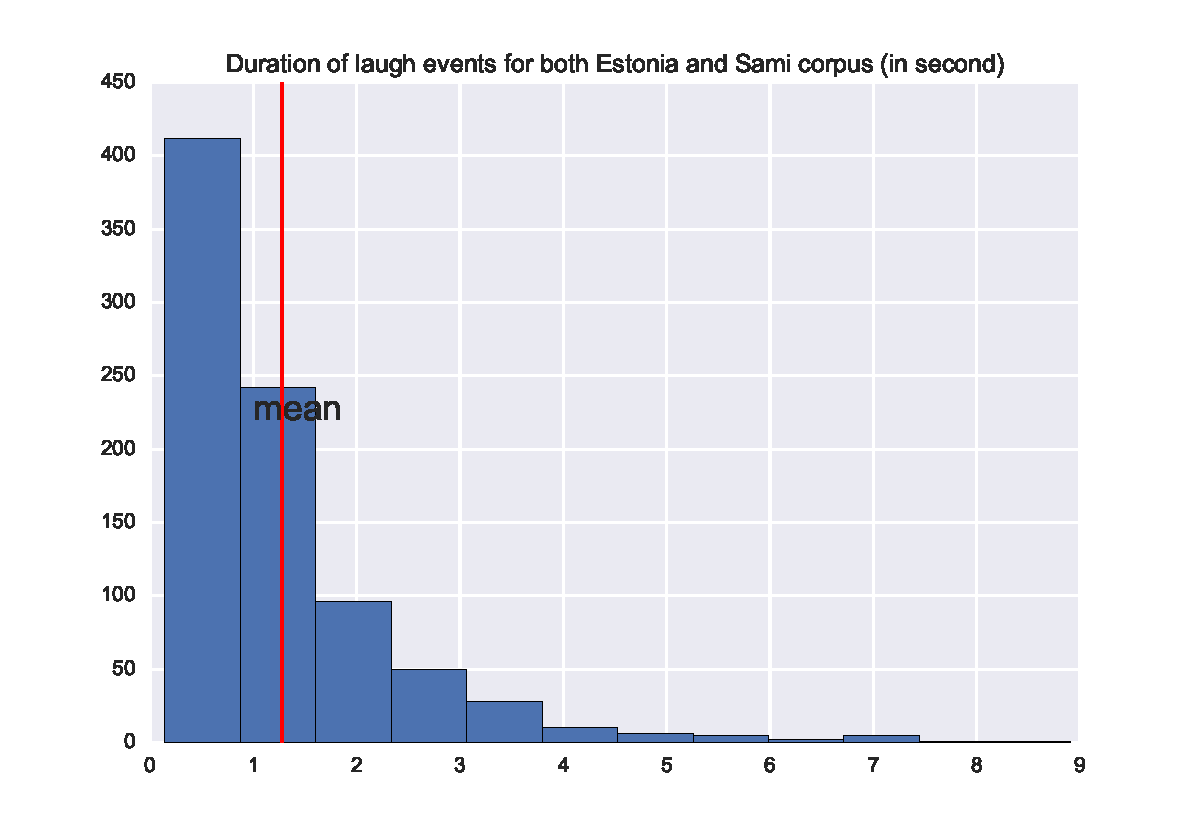
\includegraphics[width=1\linewidth]{figures/all/duration_hist.pdf}
\caption{Histogram of laugh durations in both datasets.}
\label{fig:all-duration-histogram}
\end{figure}

Figure~\ref{fig:EE-duration-histogram} shows the histogram of laugh duration in the Estonian dataset.
Most people laughed for approximately 0.8 seconds, and the laughing is rarely longer than 2 seconds.
Conversely, Figure~\ref{fig:DS-duration-histogram} indicates that in the DigiSami conversations people often laugh for longer durations (i.e ~ 1.8 seconds). Most of the events are located from 0.1 to 2 seconds and laughs longer than 4 seconds rarely occur.

\begin{figure}[!t]
\centering
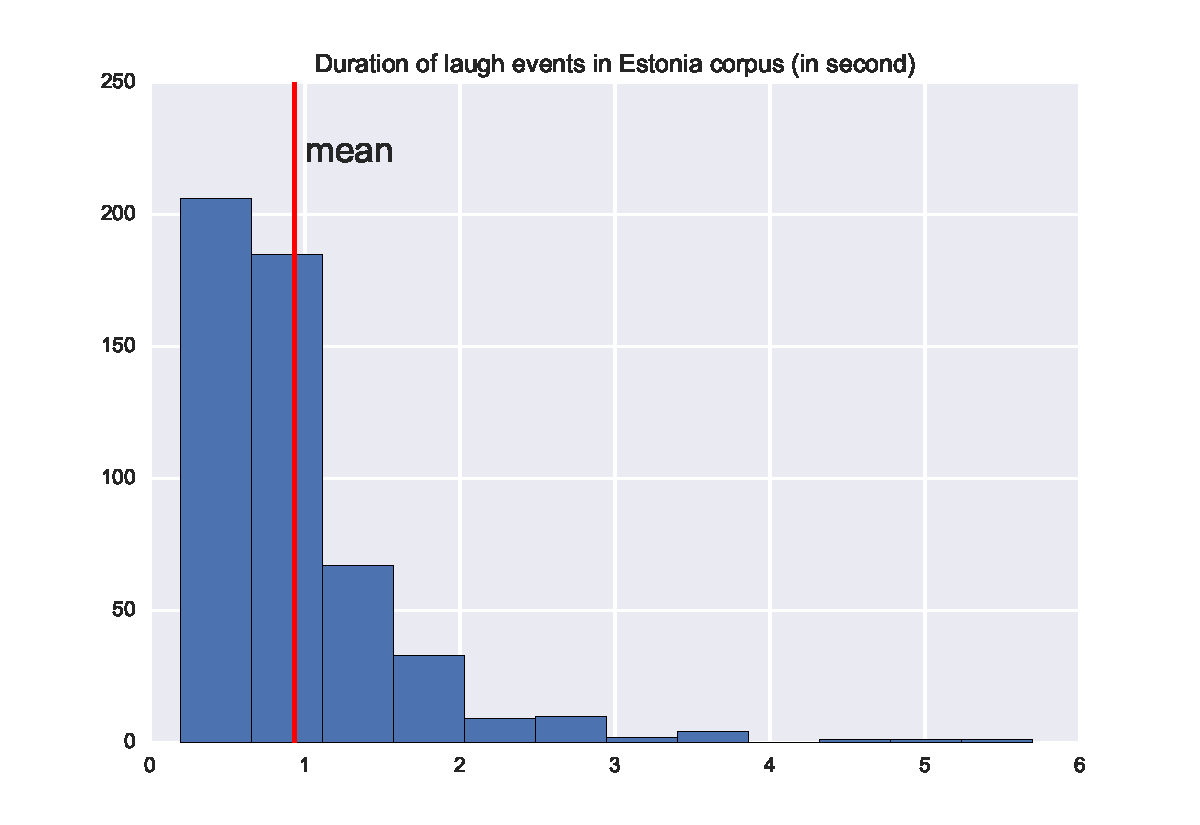
\includegraphics[width=1\linewidth]{figures/estonia/duration_hist.pdf}
\caption{Histogram of laugh durations in the Estonian dataset.}
\label{fig:EE-duration-histogram}
\end{figure}

\begin{figure}[!t]
\centering
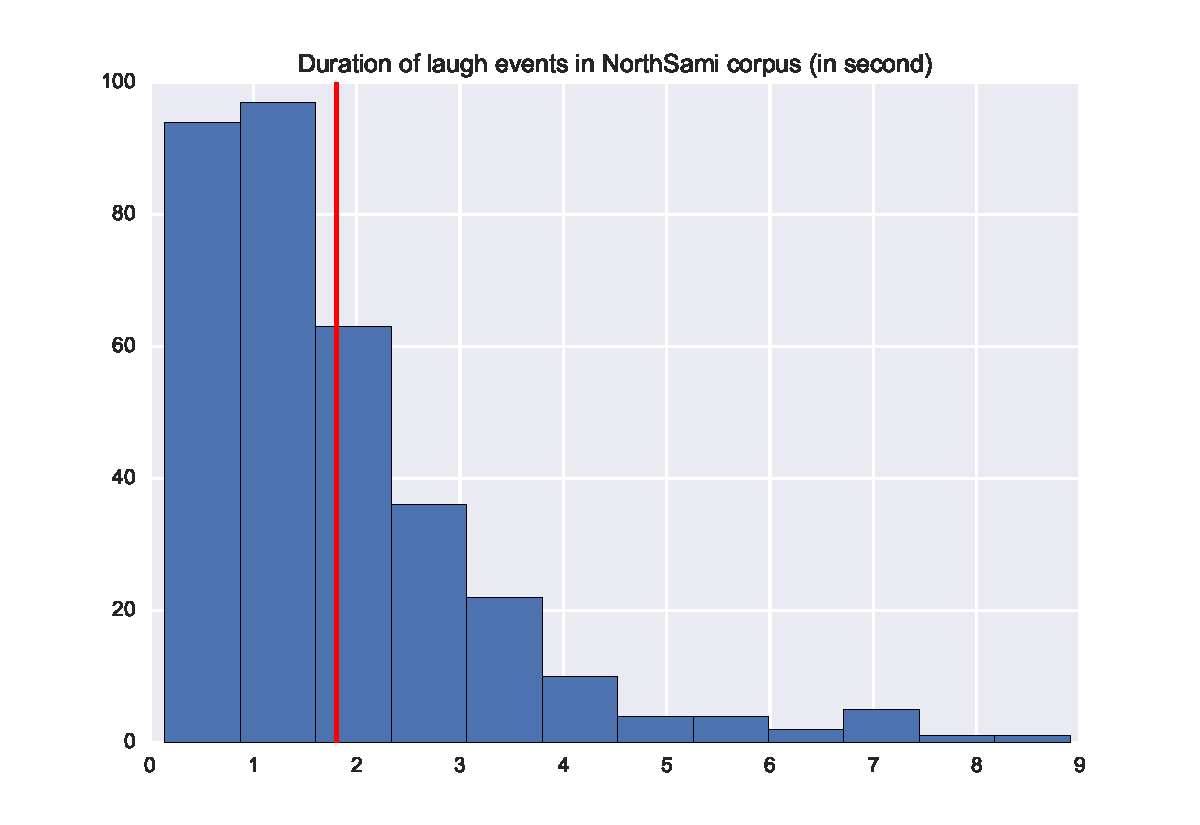
\includegraphics[width=1\linewidth]{figures/sami/duration_hist.pdf}
\caption{Histogram of laugh durations in the DigiSami dataset.}
\label{fig:DS-duration-histogram}
\end{figure}

There are significant differences between laughing events in the Estonian dataset and the DigiSami dataset, which may be the result of the following factors:
\begin{itemize}
\item The scenario of the experimental setup
\item The level of familiarity between the participants
\item Cultural differences.
\end{itemize}

\subsection{Free-laugh vs. speech-laugh}

%The box plot (Figure~\ref{fig:boxplot-laugh-events}) indicates the differences in duration between different kinds of laugh. ``st, m'' has the longest duration, but widely varies from 0.4 to 2.6 seconds. ``fl, o'' and ``fl, o, p'' rarely happened and only last for very short durations. ``fl, m''; ``fl, p''; ``fl, e''; ``st, m''; ``st, b' occurred frequently during the conversation.

Figure~\ref{fig:EE-duration-boxplot-laugh} illustrates the differences of the distribution between free-laugh (fl) and speech-laugh (st) in the Estonian dataset. We can see that speech-laugh is slightly longer than free-laugh, and more frequently appears during the conversation than free-laugh events.
However, both events are equally distributed in the DigiSami corpus (Figure~\ref{fig:DS-duration-boxplot-laugh}). Moreover, laugh events in the DigiSami data are more widely distributed than in the Estonian data, but the number of outliers in the DigiSami data is smaller than in the Estonian corpus.

\begin{figure}[!t]
\centering
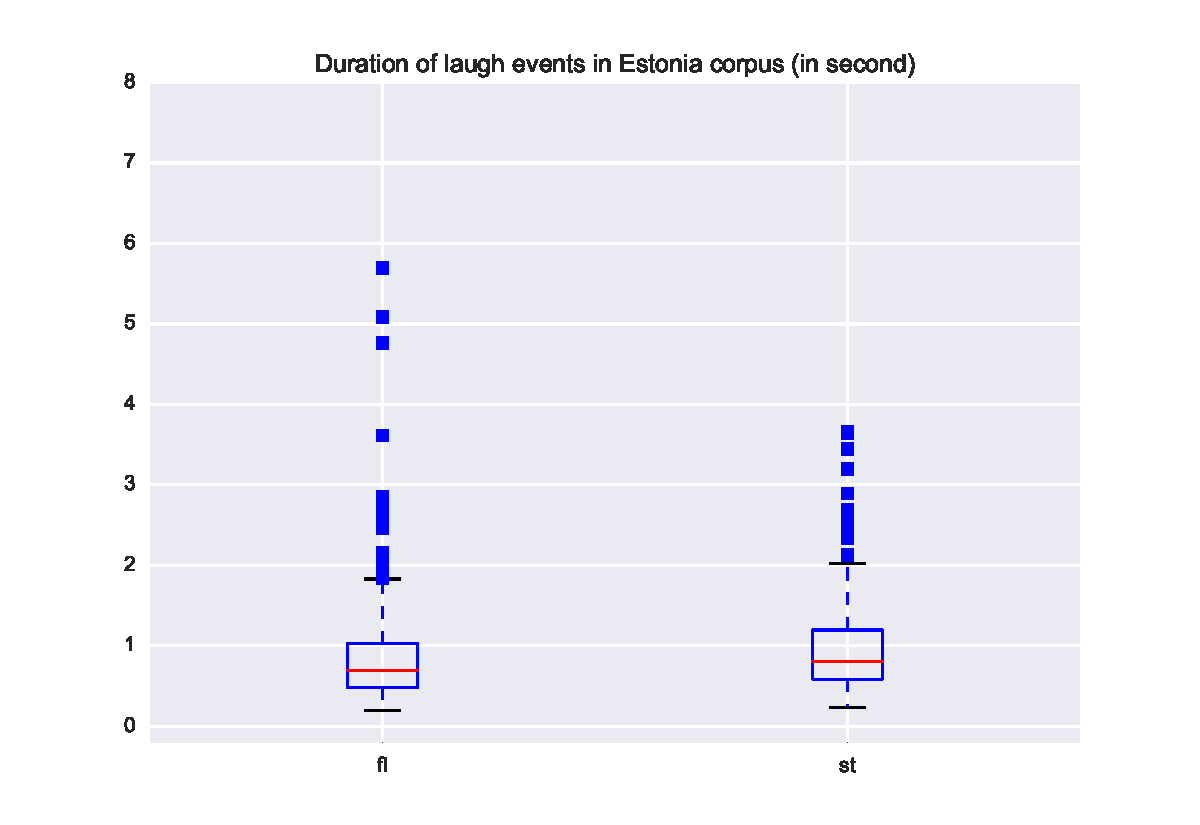
\includegraphics[width=1\linewidth]{figures/estonia/duration_boxplot_laugh.pdf}
\caption{Box plot of free-laugh vs. speech-laugh (Estonian dataset).}
\label{fig:EE-duration-boxplot-laugh}
\end{figure}

\begin{figure}[!t]
\centering
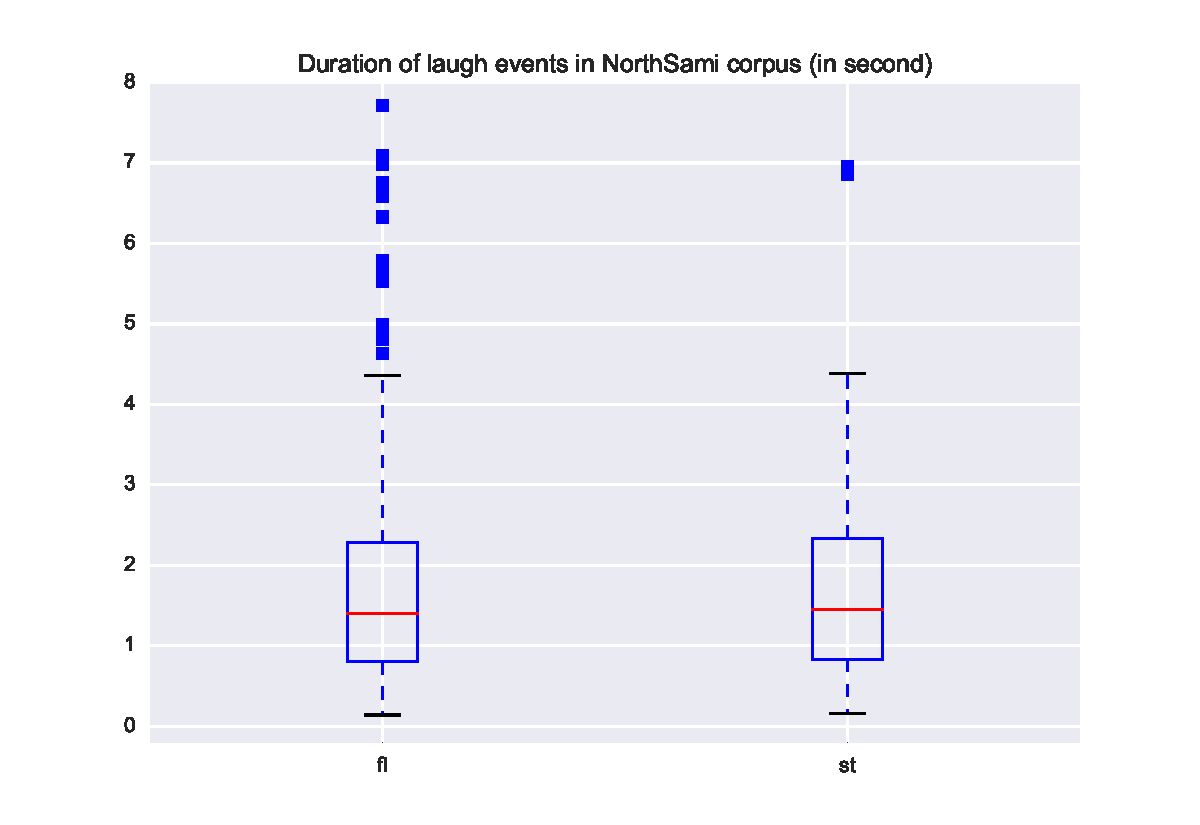
\includegraphics[width=1\linewidth]{figures/sami/duration_boxplot_laugh.pdf}
\caption{Box plot of free-laugh vs. speech-laugh (DigiSami dataset).}
\label{fig:DS-duration-boxplot-laugh}
\end{figure}

Taking into account laugh events from both Estonian and DigiSami corpora, we can see in Figure~\ref{fig:all-duration-boxplot-laugh} that free-laughs are more widely distributed than speech-laughs (i.e. longer duration range), but the average duration of free-laugh is 0.1 seconds shorter than speech-laugh. On the other hand, the number of outliers in free-laughs is greater than in speech-laughs which emphasises the unpredictable nature of free-laugh events.

\begin{figure}[!t]
\centering
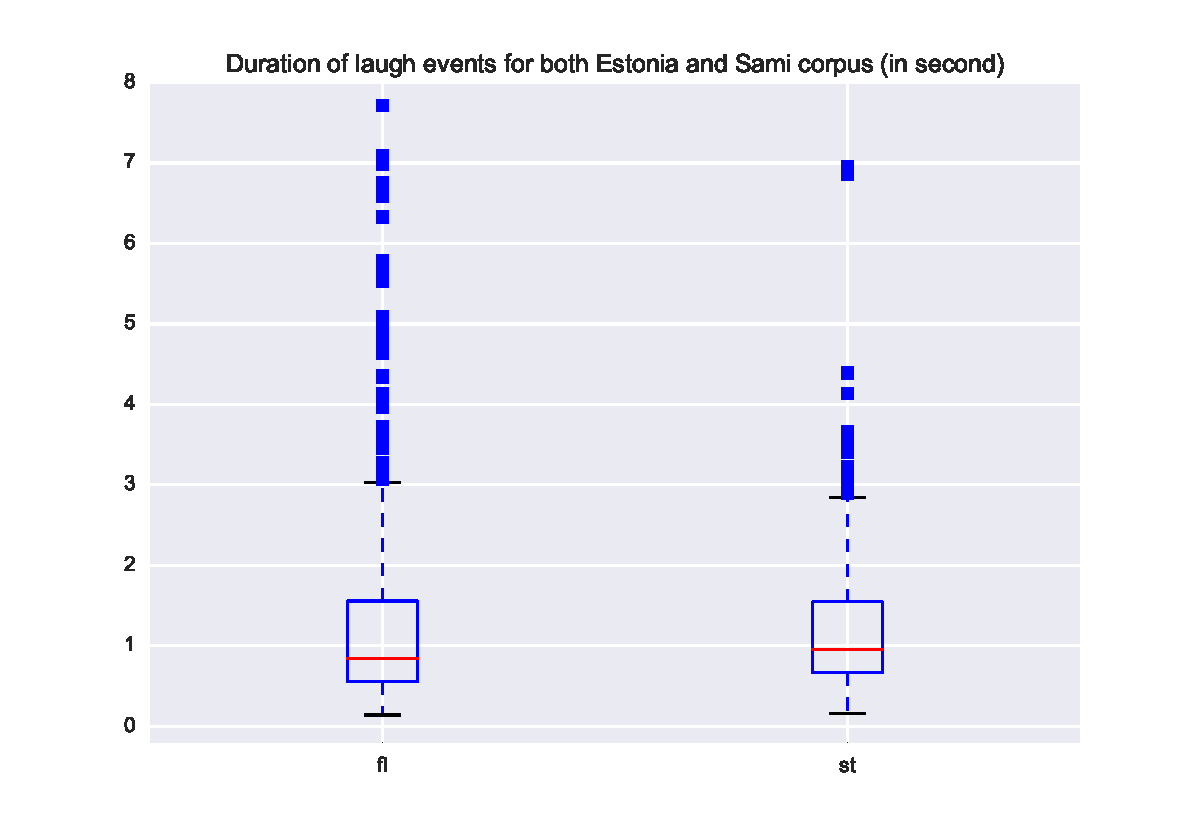
\includegraphics[width=1\linewidth]{figures/all/duration_boxplot_laugh.pdf}
\caption{Box plot of free-laugh vs. speech-laugh (combined datasets).}
\label{fig:all-duration-boxplot-laugh}
\end{figure}

\subsection{Emotional States and Laughter }

There are 7 emotional states that affect the laugh events:
\begin{itemize}
\item b: (breath) heavy breathing, smirk, sniff;
\item e: (embarrassed) speaker is embarrassed, confused,
\item m: (mirth) fun, humorous, real laughter,
\item d: (derision) mocking the partner
\item p: (polite) polite laughter showing positive
\item o: (other) laughter that doesn't fit any of the above
\end{itemize}

In general, in both corpora (Figure~\ref{fig:all-duration-boxplot-emotion}) the participants rarely laughed to mock their conversational partners, and since many conversations are between strangers, the embarrassed laugh can be frequently observed

\begin{figure}[!t]
\centering
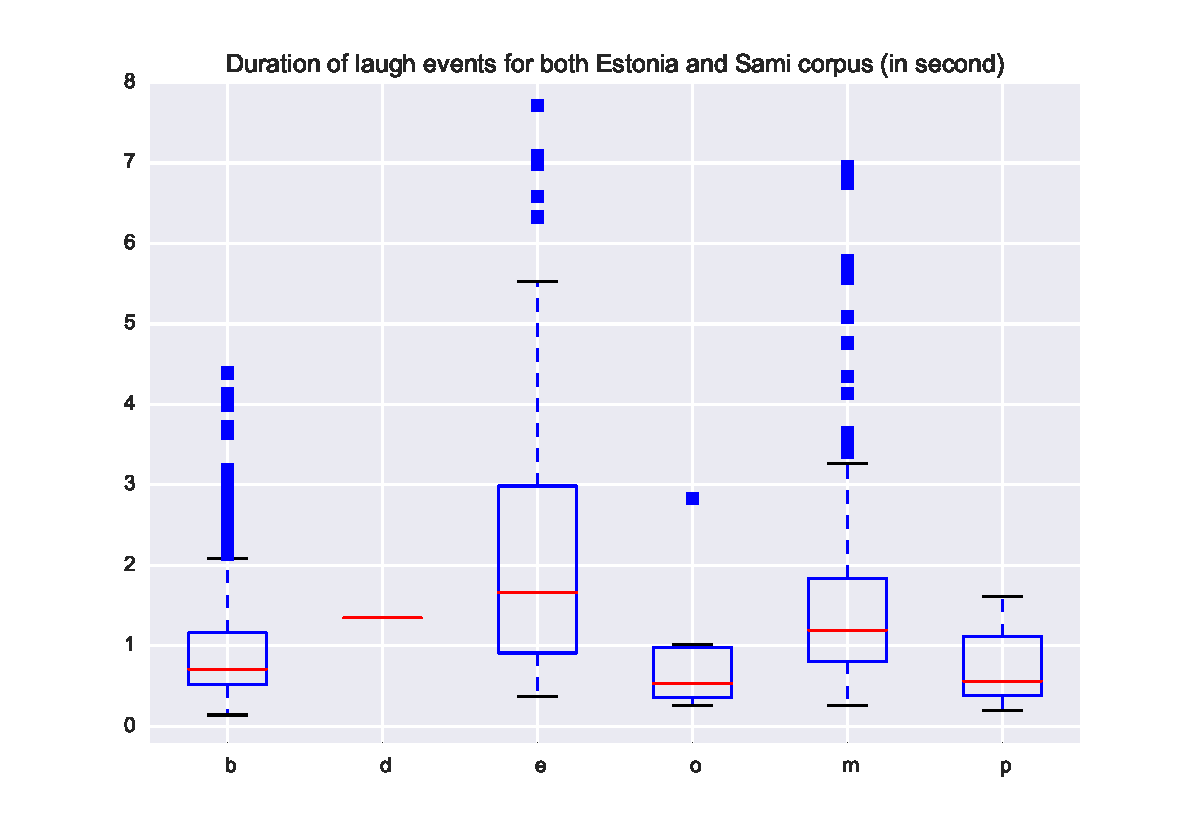
\includegraphics[width=1\linewidth]{figures/all/duration_boxplot_emotion.pdf}
\caption{Box plot of emotional states and laughter (combined datasets).}
\label{fig:all-duration-boxplot-emotion}
\end{figure}

In the Estonian corpus (Figure~\ref{fig:EE-duration-boxplot-emotion}), most of the laugh events are humorous laugh, polite laugh, embarrassed laugh and sniff laugh. However, the humorous laugh and smirk laugh are often unexpectedly longer with more outliers.

\begin{figure}[!t]
\centering
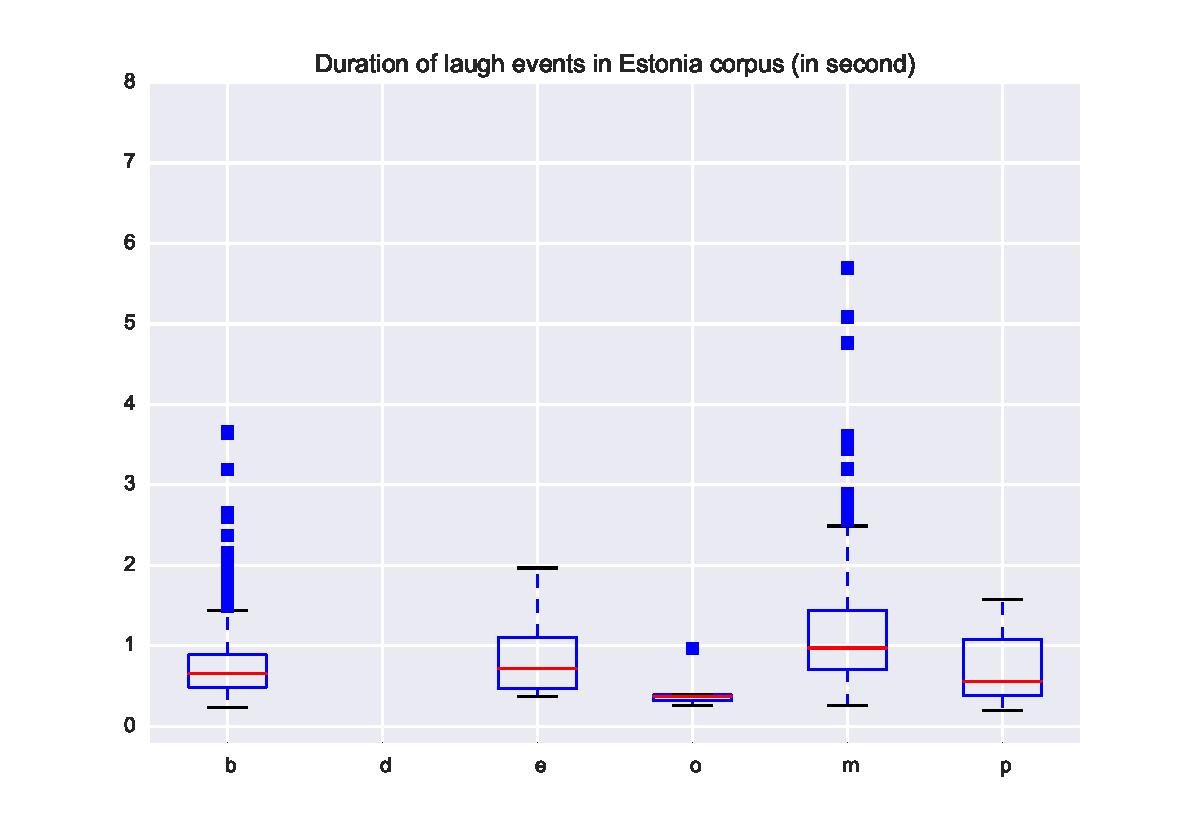
\includegraphics[width=1\linewidth]{figures/estonia/duration_boxplot_emotion.pdf}
\caption{Box plot of emotional states and laughter (Estonian dataset).}
\label{fig:EE-duration-boxplot-emotion}
\end{figure}

In the DigiSami corpus (Figure~\ref{fig:DS-duration-boxplot-emotion}), we can see many more emotional states in the laughs, and there are significant amounts of embarrassed laugh during the conversations. This is interesting because the acquainted level of the participants is generally higher than in the Estonian dataset.

\begin{figure}[!t]
\centering
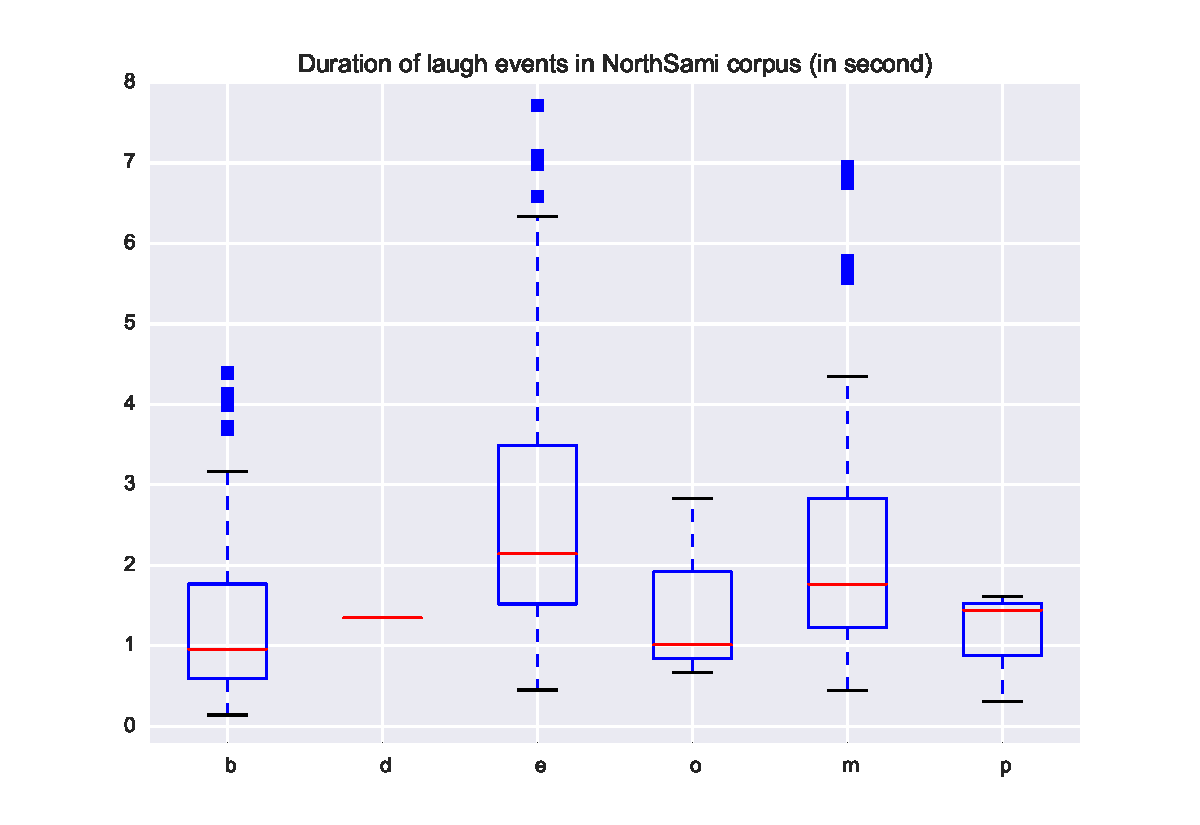
\includegraphics[width=1\linewidth]{figures/sami/duration_boxplot_emotion.pdf}
\caption{Box plot of emotional states and laughter (DigiSami dataset).}
\label{fig:DS-duration-boxplot-emotion}
\end{figure}

\subsection{Most Common Laughter Types}

In the Estonian corpus (Figure~\ref{fig:EE-duration-boxplot-types}), the most common laugh type is humorous laugh, which includes both free-laugh and speech-laugh. Conversely, embarrassed free-laugh is the most popular one in the DigiSami corpus (Figure~\ref{fig:DS-duration-boxplot-types}). Laugh is generally longer in the DigiSami dataset than the Estonian dataset. For both corpora, embarrassed laugh is often free-laugh, and humorous laugh is frequently longer with speech-laugh events.

\begin{figure}[!t]
\centering
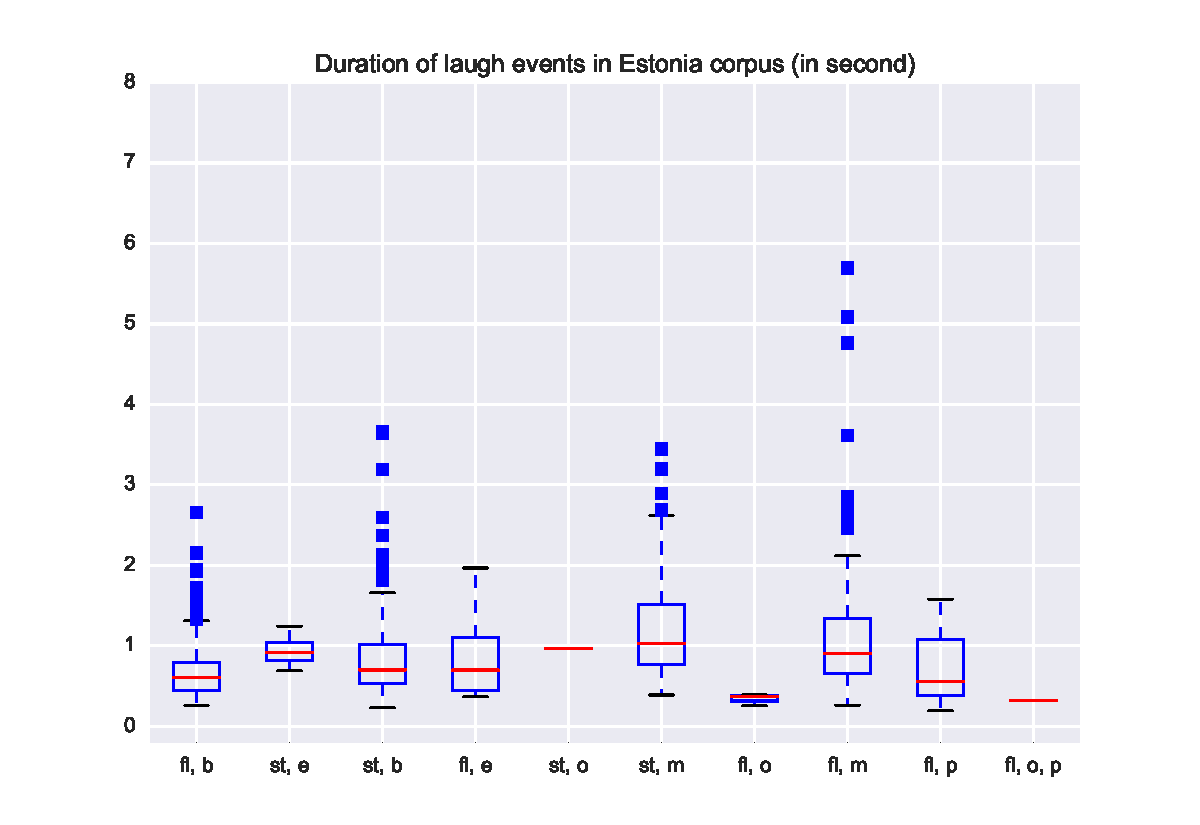
\includegraphics[width=1\linewidth]{figures/estonia/duration_boxplot_all.pdf}
\caption{Box plot of most common laughter types (Estonian dataset).}
\label{fig:EE-duration-boxplot-types}
\end{figure}

\begin{figure}[!t]
\centering
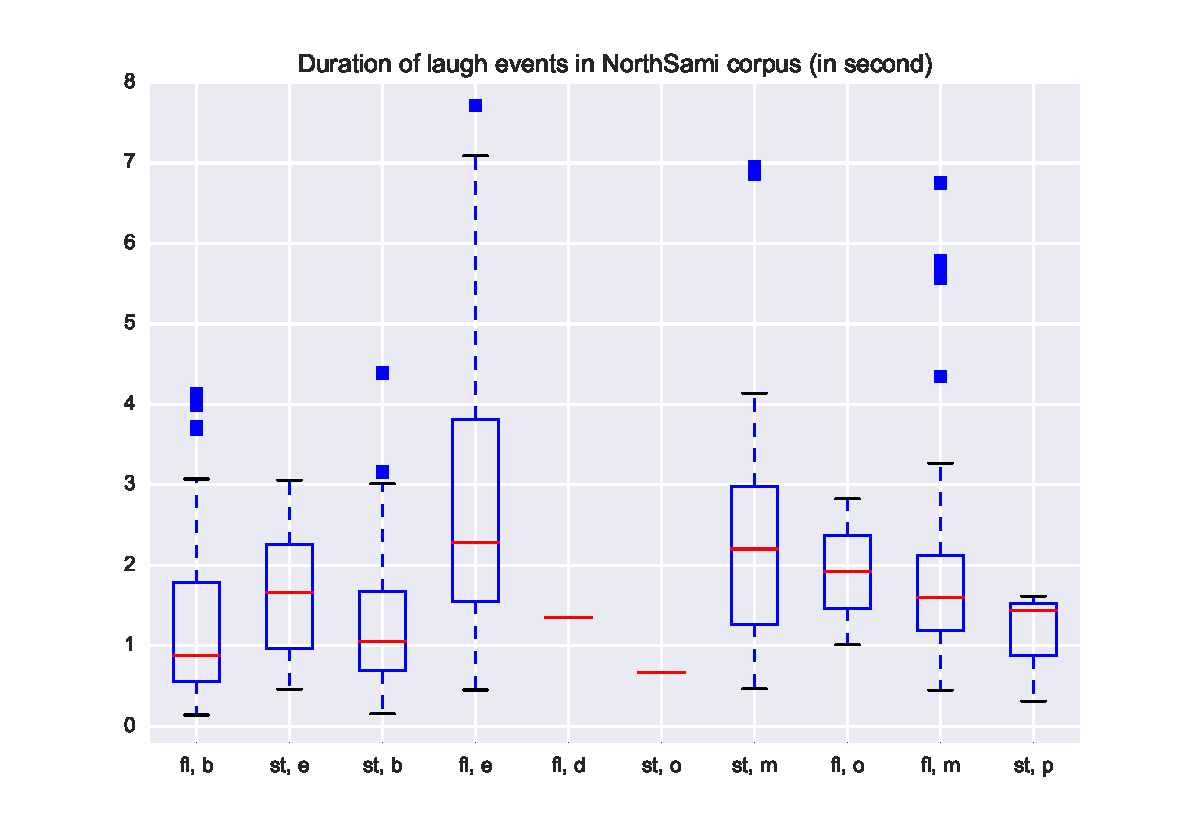
\includegraphics[width=1\linewidth]{figures/sami/duration_boxplot_all.pdf}
\caption{Box plot of most common laughter types (DigiSami dataset).}
\label{fig:DS-duration-boxplot-types}
\end{figure}

Combining both datasets (Figure~\ref{fig:all-duration-boxplot-types}), we can see that free-laugh is distributed over a longer range than speech-laugh. However, there is a contradiction between embarrassed laugh and humorous laugh. A speech-laugh which is the result of humorous action often lasts longer than a free-laugh with the same condition, and an embarrassed laugh lasts longest with free-laugh speakers.

\begin{figure}[!t]
\centering
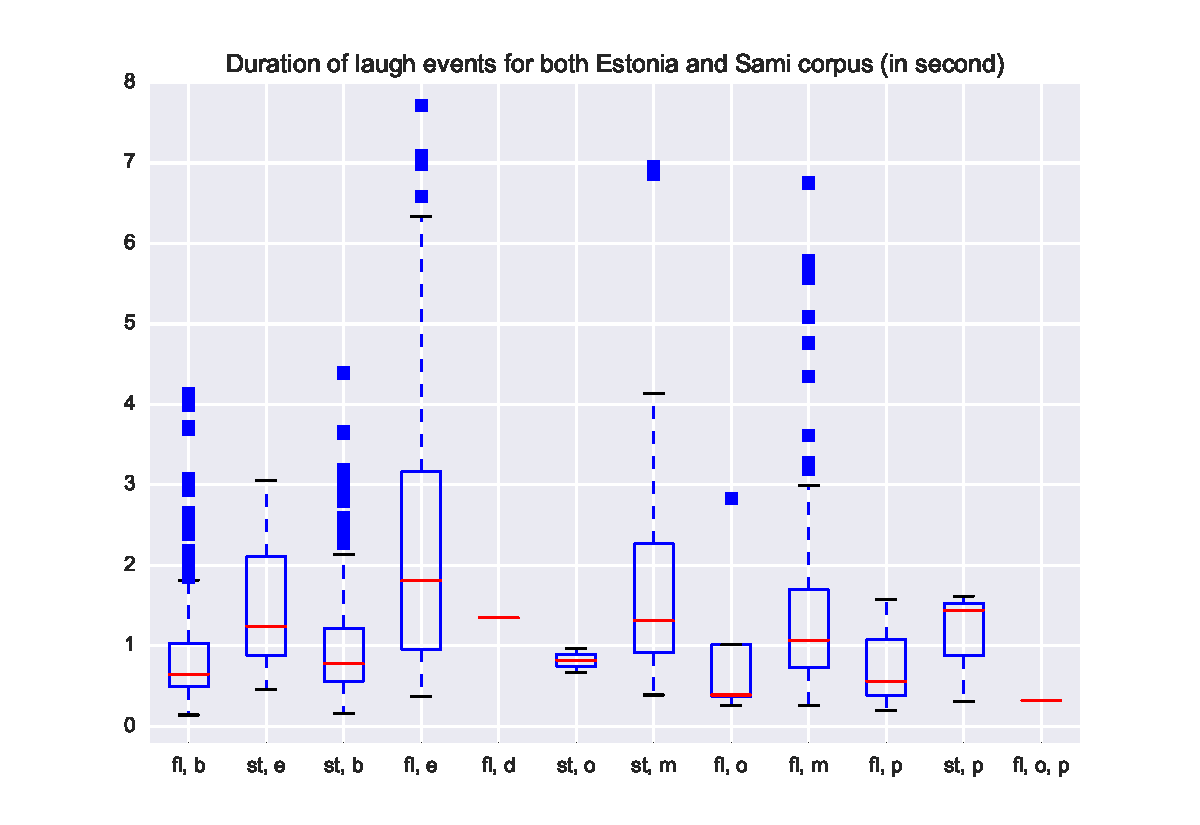
\includegraphics[width=1\linewidth]{figures/all/duration_boxplot_all.pdf}
\caption{Box plot of most common laughter types (combined datasets).}
\label{fig:all-duration-boxplot-types}
\end{figure}


\section{Acoustic Analysis}
\label{sec:acoustic-analysis}

Following the previous research, we hypothesize that the different laughter types in our data differ in their acoustic properties, such as pitch, formants and intensity, and also duration. In the following acoustic analysis, only the basic and most common laughter types, mirthful (m), breath (b) and uncertain/embarrassed (e) and polite (p) in the Estonian data are included, occurring either in free-laughters (fl) or in speech-laughs (st). The analyses have been made with different Praat scripts and further processed for min/max/ave/std values. The scripts were originally produced by Mietta Lennes, Shigeto Kawahara (intensity), and Jonas Lindh (F0).

Our analysis of the acoustic features showed various differences in the investigated laughter types. To compare the results of the acoustic analyses, we calculated average values from the 3-4 most common types (breath, embarrassed, mirth, polite) of male and female informants separately.

\subsection{Most Common Laughter Types}

The most common laughter types by male and female participants are shown in Figure~\ref{fig:m-f-digisami} for the DigiSami corpus and in Figure~\ref{fig:m-f-estonian} for the Estonian corpus.
As can be seen, in both corpora female participants produce more laughter signals than men, usually about twice as many. An exception is free-laughing breath types where the ratio is the other way round: this is the typical laugh type for the men in the DigiSami data. It is also interesting that females produce embarrassed and uncertain speech-laughs about four time as many as male participants, being the most typical laugh-type for women in the DigiSami data.

\begin{figure}[!t]
\centering
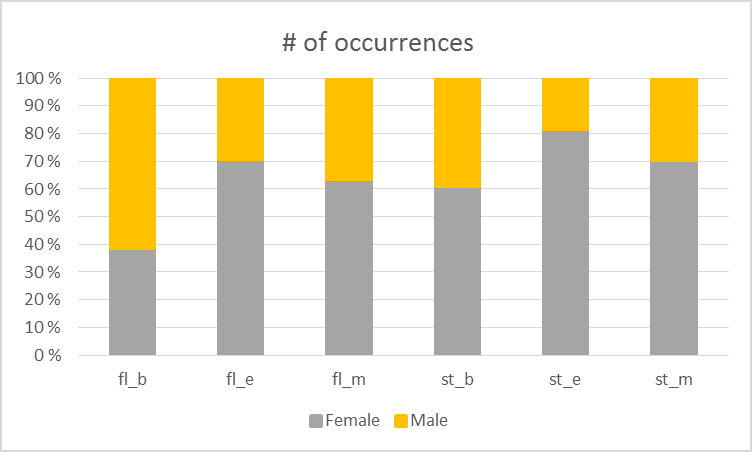
\includegraphics[width=1\linewidth]{images/M-F-DigiSami.png}
\caption{Male and Female Laughter in DigiSami Corpus.}
\label{fig:m-f-digisami}
\end{figure}

\begin{figure}[!t]
\centering
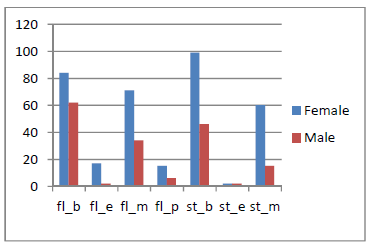
\includegraphics[width=1\linewidth]{images/M-F-MINT.png}
\caption{Male and Female Laughter in Estonian MINT Corpus.}
\label{fig:m-f-estonian}
\end{figure}

In the Estonian data, the most common laughter type is the breathy type both in free-laugh and speech-laugh, as shown in Figure~\ref{fig:m-f-estonian}. Also in the Estonian data, female participants produced remarkably more laughter than male participants.

\subsection{F0 Values of Different Laughter Types}

Figures~\ref{fig:f0-digisami} and~\ref{fig:f0-estonian} show F0 (pitch) values which were extracted with different ranges for male (75-400Hz) and female (100-500Hz) informants; thus comparison of male and female average values is not adequate. However, in the DigiSami data it was clear that the F0 in free-laughter types was higher than F0 in speech-laughter for both male and female informants, which accords e.g. with \cite{Truong:vanLeeuwen:07}. In the Estonian data the polite free-laugh had the highest pitch of all laughter types, both for female and male participants. The free-laugh types of male participants were clearly higher than the speech-laughs. Generally, there were no big differences between F0 values of all laughter types.

\begin{figure}[!t]
\centering
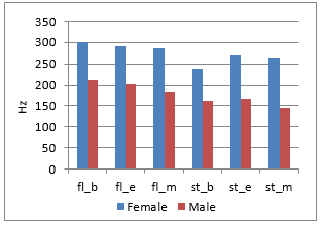
\includegraphics[width=1\linewidth]{images/F0-DigiSami.png}
\caption{F0 Values for Male and Female Laughter in DigiSami Corpus.}
\label{fig:f0-digisami}
\end{figure}

\begin{figure}[!t]
\centering
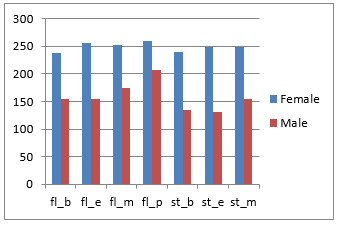
\includegraphics[width=1\linewidth]{images/F0-MINT.png}
\caption{F0 Values for Male and Female Laughter in Estonian Corpus.}
\label{fig:f0-estonian}
\end{figure}

\subsection{Average Duration of Different Laughter Types}

Figures~\ref{fig:duration-digisami} and~\ref{fig:duration-estonian} depict the average durations of the laugh types. In the DigiSami data, there were big differences in duration between the laugher types: durations of embarrassed laughs were significantly longer (2.1-3.2 seconds) than all other types for both male and female informants, and breath laughs were the shortest (1.1-1.4 seconds). The durations in the Estonian data were very different compared to the DigiSami data: the longest laughter bout in the Estonian data was only 1.3 seconds, while in the DigiSami data the longest was 3.2 seconds. One explanation for this significant difference could be the different interaction situation: the Estonian participants met each other for the first time, while in the DigiSami data the participants knew each other beforehand, thus the laughter bouts were longer.

\begin{figure}[!t]
\centering
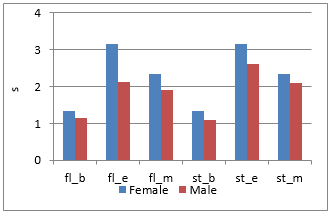
\includegraphics[width=1\linewidth]{images/Duration-DigiSami.png}
\caption{Durations of Male and Female Laughter in DigiSami Corpus.}
\label{fig:duration-digisami}
\end{figure}

\begin{figure}[!t]
\centering
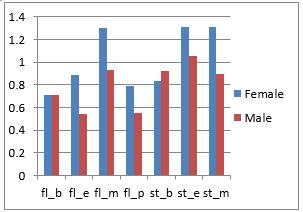
\includegraphics[width=1\linewidth]{images/Duration-MINT.png}
\caption{Durations of Male and Female Laughter in Estonian Corpus.}
\label{fig:duration-estonian}
\end{figure}

The Estonian data had the longest laughter bouts in mirthful types, while the polite and breathy types were the shortest. Both in the Estonian and DigiSami data, the embarrassed speech-laugh was the longest produced by both female and male participants.

However, our data did not support the findings of Nwokah et al. \cite{Nwokah:ea:99} since free-laughter in our data was not significantly longer than speech-laughs. This may be due to the different interaction activities: our data records people conversing in fairly equal situations compared with a mother and child care-giving interaction.

\subsection{Intensity of Different Laughter Types}

Both in the DigiSami and Estonian data the intensity of different laughter types was rather similar in all laughter types, as shown in Figures~\ref{fig:intensity-digisami} and~\ref{fig:intensity-estonian}. No significant differences occurred between the different laughter types, but the most surprising difference in the DigiSami data was that the average intensity with female informants was generally bigger than with males, while in the Estonian data many laughter types had higher intensity with male informants.

\begin{figure}[!t]
\centering
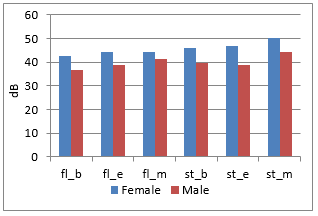
\includegraphics[width=1\linewidth]{images/Intensity-DigiSami.png}
\caption{Intensity of Male and Female Laughter in DigiSami Corpus.}
\label{fig:intensity-digisami}
\end{figure}

\begin{figure}[!t]
\centering
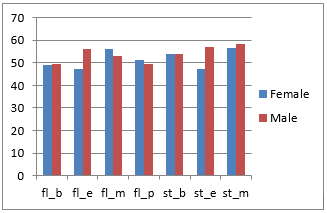
\includegraphics[width=1\linewidth]{images/Intensity-MINT.png}
\caption{Intensity of Male and Female Laughter in Estonian Corpus.}
\label{fig:intensity-estonian}
\end{figure}

%%%%%%%%%%%%%%%%%%%%%%%%%%%%%%%%%%%%%%%%%%%%%%%%%%%%%%%%%%%%%%%%%%%%%%
%%% Section 7
\section{Multi-modal laughter analysis}
\label{sec:multi-modal laughter analysis}

%%%%%%%%%%%%%%%%%%%%%%%%%%%%%%%%%%%%%%%%
\subsection{Topic annotations}
\label{sec:topic-annotations}
Our first investigation aims for explaining how conversational topic evolved in different cultures and its correlation to laughter events.
The dialogues are segmented and annotated the conversational semantics by our expert, in order to achieve comparative results among different copora, we translated all the conversations to English as well as the topic annotations. An example of the annotation is shown in Table~\ref{tab:diagsum}, the summarization provide detail information of the discussion, as a results, they aren't constrained into categories as other approach. This strategy proposed both opportunity and challenges. The researcher can have closer understanding of the topic flow during the conversation, the pattern in topic switching, speaker behaviour are clearly emerged from the dialogues. On the drawbacks, the approach halt significant difficulties in modeling topic for automated system, since the descriptions are different among the files even though they could indicate the same topic of discussion. In this section, we describe our approach to normalize the summarization into a limited number of group in which emerges the transitions between latent topics.

\begin{table}[h]
\begin{center}
\begin{tabular}{|l|l|p{4cm}|}
\hline \bf Start (s) & \bf End (s) & \bf Summarization \\ \hline
13 & 18 & greetings, introductions \\ \hline
18 & 27 & occupations, studying language technology \\ \hline
27 & 64 & language technology at the university \\ \hline
64 & 200 & specializing fields in LT \\ \hline
200 & 278 & spoken dialogue systems \\ \hline
278 & 328 & morphological analysis and synthesis, topics in LT \\
\hline
\end{tabular}
\end{center}
\caption{The summarization of the dialogues within the ``C\_16\_MM\_15\_16'' conversation from Estonian first encounter dataset}
\label{tab:diagsum}
\end{table}

\subsubsection{Text preprocessing for topic clustering}
During the tokening process, we figure out that aggressively normalization the token give the best topic clusters. This strategy involves the removal of stop-words, punctuations, out-of-dictionary words, and the stemming. It is notable that stemming is more efficient than lemmatizing in our case since lemmatization will introduce more duplication (e.g. studying and study, or introduction and introducing), conversely, stemming significantly reduces the vocabulary size which is important for a small corpus. As we want to encourage the most compact representation of multiple descriptions among different conversations, we choose \textit{term frequency – inverse document frequency} (tf-idf) to extract the vector representation of each word. For each term $t$ in document $d$, the term-frequency (tf) score is calculated as follow:
\[
{\displaystyle \mathrm {tf} (t,d)= {\frac {f_t}{|d|}}},
\]
where, $f_t$ is number of times term $t$ appears in a document and $|d|$ is total number of term in document $d$. Additional, the inverse-document-frequency (idf) is estimated by
\[
idf(t) = log(\frac{|D|}{|D_t|}),
\]
where, $|D|$ is the total number of documents in our corpus, and $|D_t|$ is the number of documents that contain term $t$.
Finally, the weight for term $t$ is obtained by:
\[
{\displaystyle \mathrm {tfidf} (t,d,D)=\mathrm {tf} (t,d)\cdot \mathrm {idf} (t,D)}
\]

\subsubsection{Topic clustering}
Each of the topics is represented as a collection of ranked words from the extracted vocabulary, this task can be interpreted as clustering the word vectors into $N$ most distinguishable clusters, where $N$ is a heuristic number for a predefined number of topics. We compare the performance of traditional \textit{K-mean} clustering and \textit{latent Dirichlet allocation} (LDA)
% \cite{Blei:LDA}
for this task.

The K-mean algorithm randomly picks $N$ initial positions for topics in the word vector space, then it repeats the assignment and updates step to minimizes the within-cluster sum of squares objective for all clusters, since the algorithm converges to a different solution for each initialization, we performed it twelve times then selecting the best result.

LDA starts from the assumption that each document is a mixture of a given number of topics
% \cite{Blei:LDA}
, as a result, each word in the response is generated by sampling from one of the document's topic. The model can be described by this joint distribution
\begin{equation}
\begin{aligned}
P({\boldsymbol{W}},{\boldsymbol{Z}},{\boldsymbol{\theta }},{\boldsymbol{\varphi}};\alpha ,\beta ) &= \prod _{i=1}^{K}P(\varphi _{i};\beta ) \cdot \prod _{j=1}^{M}P(\theta _{j};\alpha ) \cdot \\
    & \prod _{t=1}^{N}P(Z_{j,t}\mid \theta _{j})P(W_{j,t}\mid \varphi _{Z_{j,t}}),
\end{aligned}
\end{equation}
where, $\alpha$ and $\beta$ encapsulate prior knowledge of the topic occurrences and word occurrences in given topic. $\theta$ and $\varphi$ are the learned Dirichlet captured the distribution of topics in a given document, and distribution of words in every topic. Training data is introduced via $\boldsymbol{W}$ and $\boldsymbol{Z}$ which are all words appeared in the document and topics of every word in the corpus. By modeling this joint distribution, we trace back the probabilistic generative process that each document is produced, hence, the technique is designed to cope with the uncertainty and ambiguity of topic modeling.

\begin{figure*}[t]
  \centering
  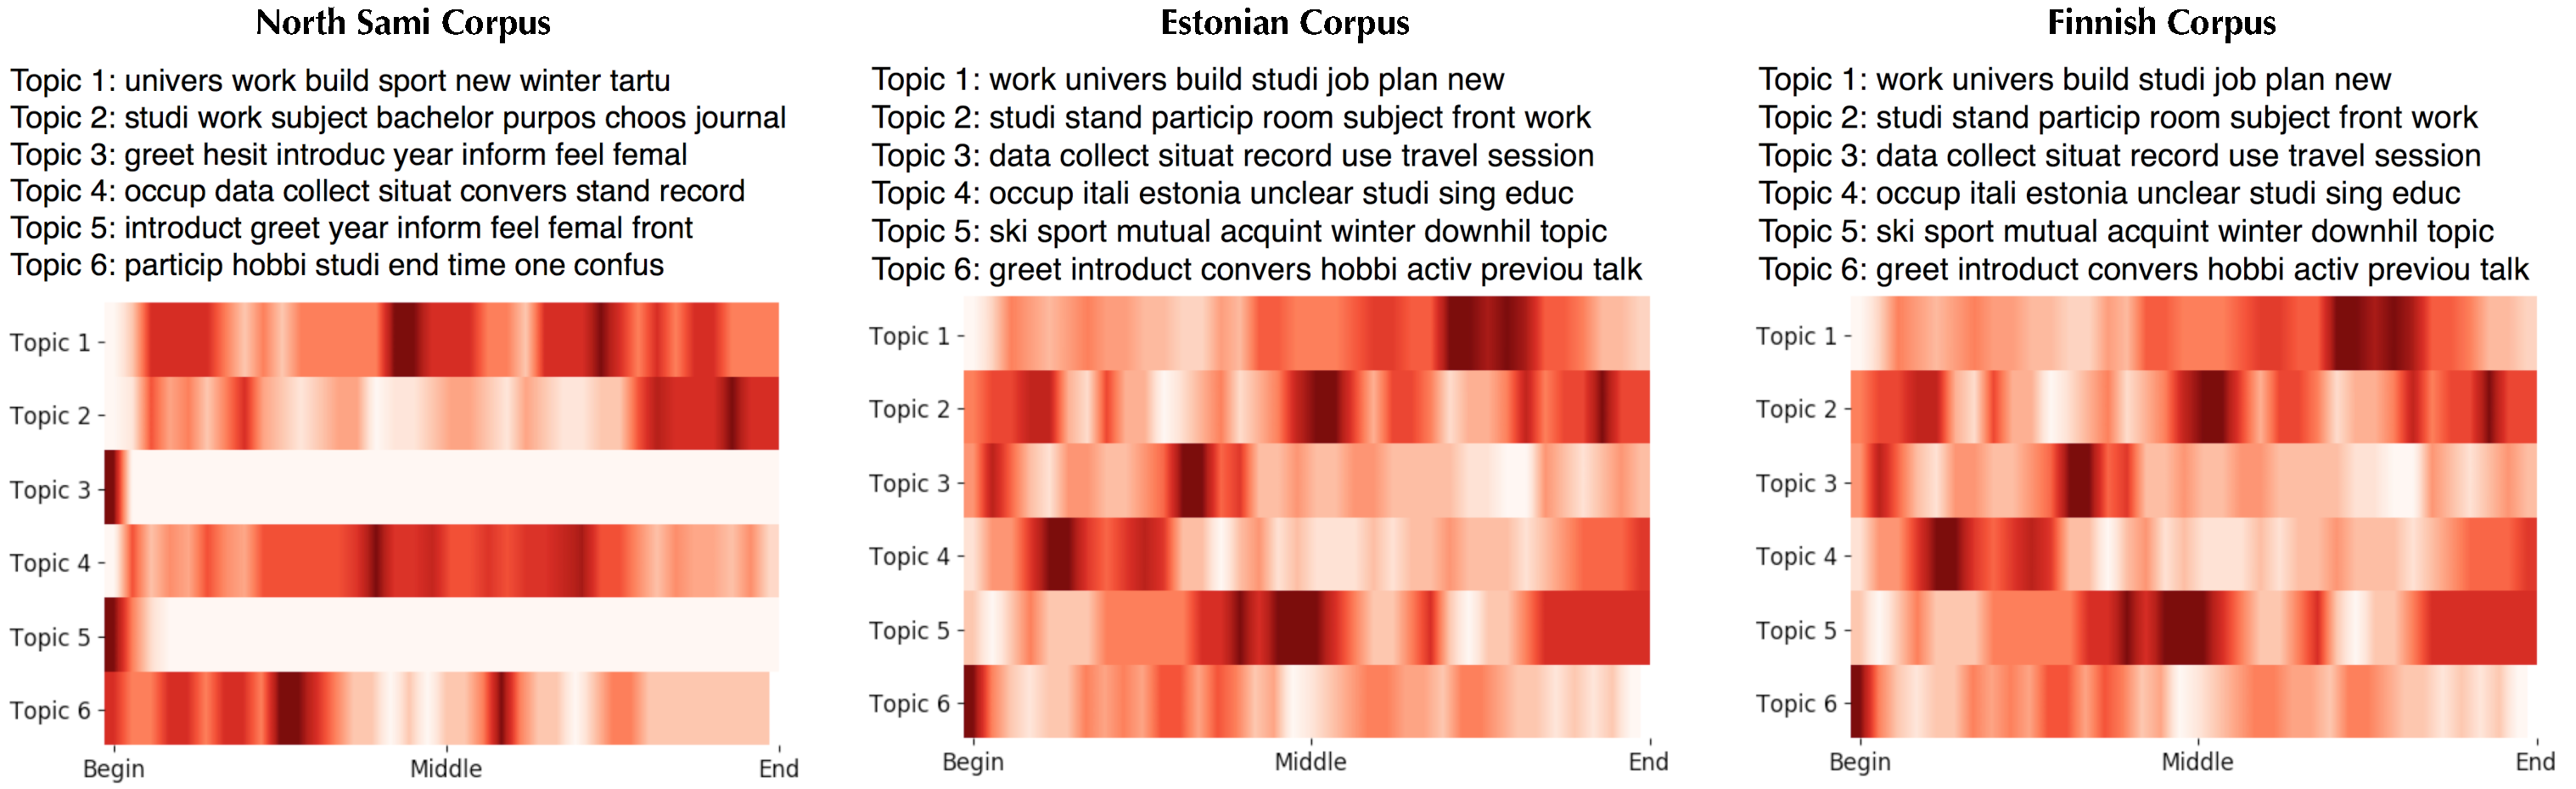
\includegraphics[width=\linewidth]{figures/lda_topic_clustering.pdf}
  \caption{Distribution during the conversation of extracted topic clusters from LDA, a comparison among North Sami, Estonian and Finnish copora.}
  \label{fig:lda_topic}
\end{figure*}
Figure~\ref{fig:lda_topic} emphasizes the different between K-mean and LDA, K-mean provides more overlap topics in both semantic and temporal aspects (e.g. Topic 3 and 5). The topics detected by LDA are often discussed for a specific period of time during the conversation, and each topic has a separated concentration region in the dialogue (e.g. topic 1 is often discussed at the end of the conversation while topic 4 is often after the greetings and introductions). In this experiment, we selected six topics as a result of a trial-error process, the number of topics is increased from two until there is significant overlapping in both the top representative terms and time spectrum.

From Figure~\ref{fig:lda_topic}, we can see that the discussion in Finnish dataset is more narrow to a certain topic (i.e. topic 2 is overwhelmed). Furthermore, the time distribution is also different, for instance, topic 6 in both datasets is often about the introductions, today's activities and previous conversation within the first encounter, however, the Estonian discussion are often happened earlier during the dialogue.

%%%%%%%%%%%%%%%%%%%%%%%%%%%%%%%%%%%%%%%%
\subsection{Visual presentation of speakers}

\begin{figure}
  \centering
  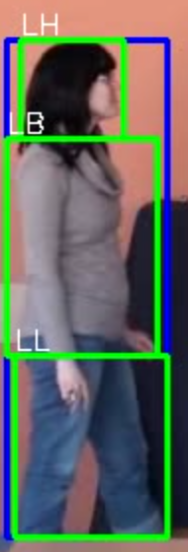
\includegraphics[width=0.18\linewidth]{images/boundingbox.png}
  \caption{The bounding box is extracted for each speaker, and segmented into head, body and legs movement.}
  \label{fig:bb}
\end{figure}

In order to extract visual features, we use bounding box which keeps tracking the marginal movements of individual speakers as shown in Figure~\ref{fig:bb}. However, the bounding box itself is just a list of integers at a given time-stamp, since we need to extract the event within a period of time, we calculate the delta and delta-delta features for a sequence of bounding box within a fixed time windows. Those features reflect the changing over time of these boundaries and the acceleration speed of these changes,
\[
d_t = \frac{\sum_{n=1}^N n\cdot(b_{t+n} - b_{t-n})}{2 \sum_{n=1}^{N} n^2},
\]
where $d_t$ is the delta features, $b_{(.)}$ is the bounding box at time $(.)$ and $N$ is the window size which is $9$ in our case. The algorithm slides the window over time axis to estimate the differences in bounding boxes. We then take the mean of the changing of all four corner that defines a bounding box to estimate the overall changing for each body parts.

Since the auditory signal is strongly speaker dependence, transforming raw waveform into time-frequency domain would result high-dimensional spectrogram which is a huge drawback for small corpus. We use the laughter annotation as a representative features for the audio signals. The annotation divide laughing events into two main categories:
\begin{itemize}
    \item Free laughter: laughter without speaking simultaneously
    \item Speech laugh: laughter and speech combined
\end{itemize}


%%%%%%%%%%%%%%%%%%%%%%%%%%%%%%%%%%%%%%%%
\subsection{Time synchronization of multi-modal features}
Our dialogues have been recorded in both video and audio which are provided in different sampling rate. The videos is recorded at 25 frames per second, while the wave file is captured at the rate of 44100 Hz. It is important to scale the two types of signal into a universal time scale for synchronization. As a result, we divide and each conversation into discrete units $u = 0.01 (second)$, this number was carefully selected to be sufficiently small that all the video actions and speech events are longer. Given an $n^{th}$ happened event, we calculate the time bucket of the event as follow
\[
    t_{new} = \mathrm{floor}\bigg(\frac{n}{f \cdot u}\bigg),
\]
where $f$ is the sampling rate of the given modality. It is essential that an event happens during a period of time which is specified by the starting and ending time-stamp, and the study of collaboration between modality involves detecting the co-occurred events. We defined two events is overlapping if and only if the following condition is satisfied
\begin{equation}
\begin{aligned}
    max(0, min(e_1, e_2) - max(s_1, s_2)) \geq \\
    max(e_1 - s_1, e_2 - s_2),
\end{aligned}
\end{equation}
where $(s_1,e_1)$ is the starting and ending time of the first event, and vice versa $(s_2, e_2)$ for the second event.

%%%%%%%%%%%%%%%%%%%%%%%%%%%%%%%%%%%%%%%%
\subsection{Multi-modal perspective of laughter}
Figure~\ref{fig:multimodal} illustrates the relation between multi-modal and conversational topic. We can see that the clear tendency of strong movement at the beginning of each dialogue, since most of the participants start with a handshake. Furthermore, the movements are more intense in the area where the speakers changing the topics more frequently as indicated by the red ellipses. It is also notable that the participants often laugh when talking about topic 3 - ``data collection situation''(the green), but the events rarely happen for topic 6 - ``greetings, today activities, previous interview''(the yellow). It is likely that the conversations that involve female participant are more active which is signed by a higher amount of laugh and frequent movements.
\begin{figure*}[t]
  \centering
  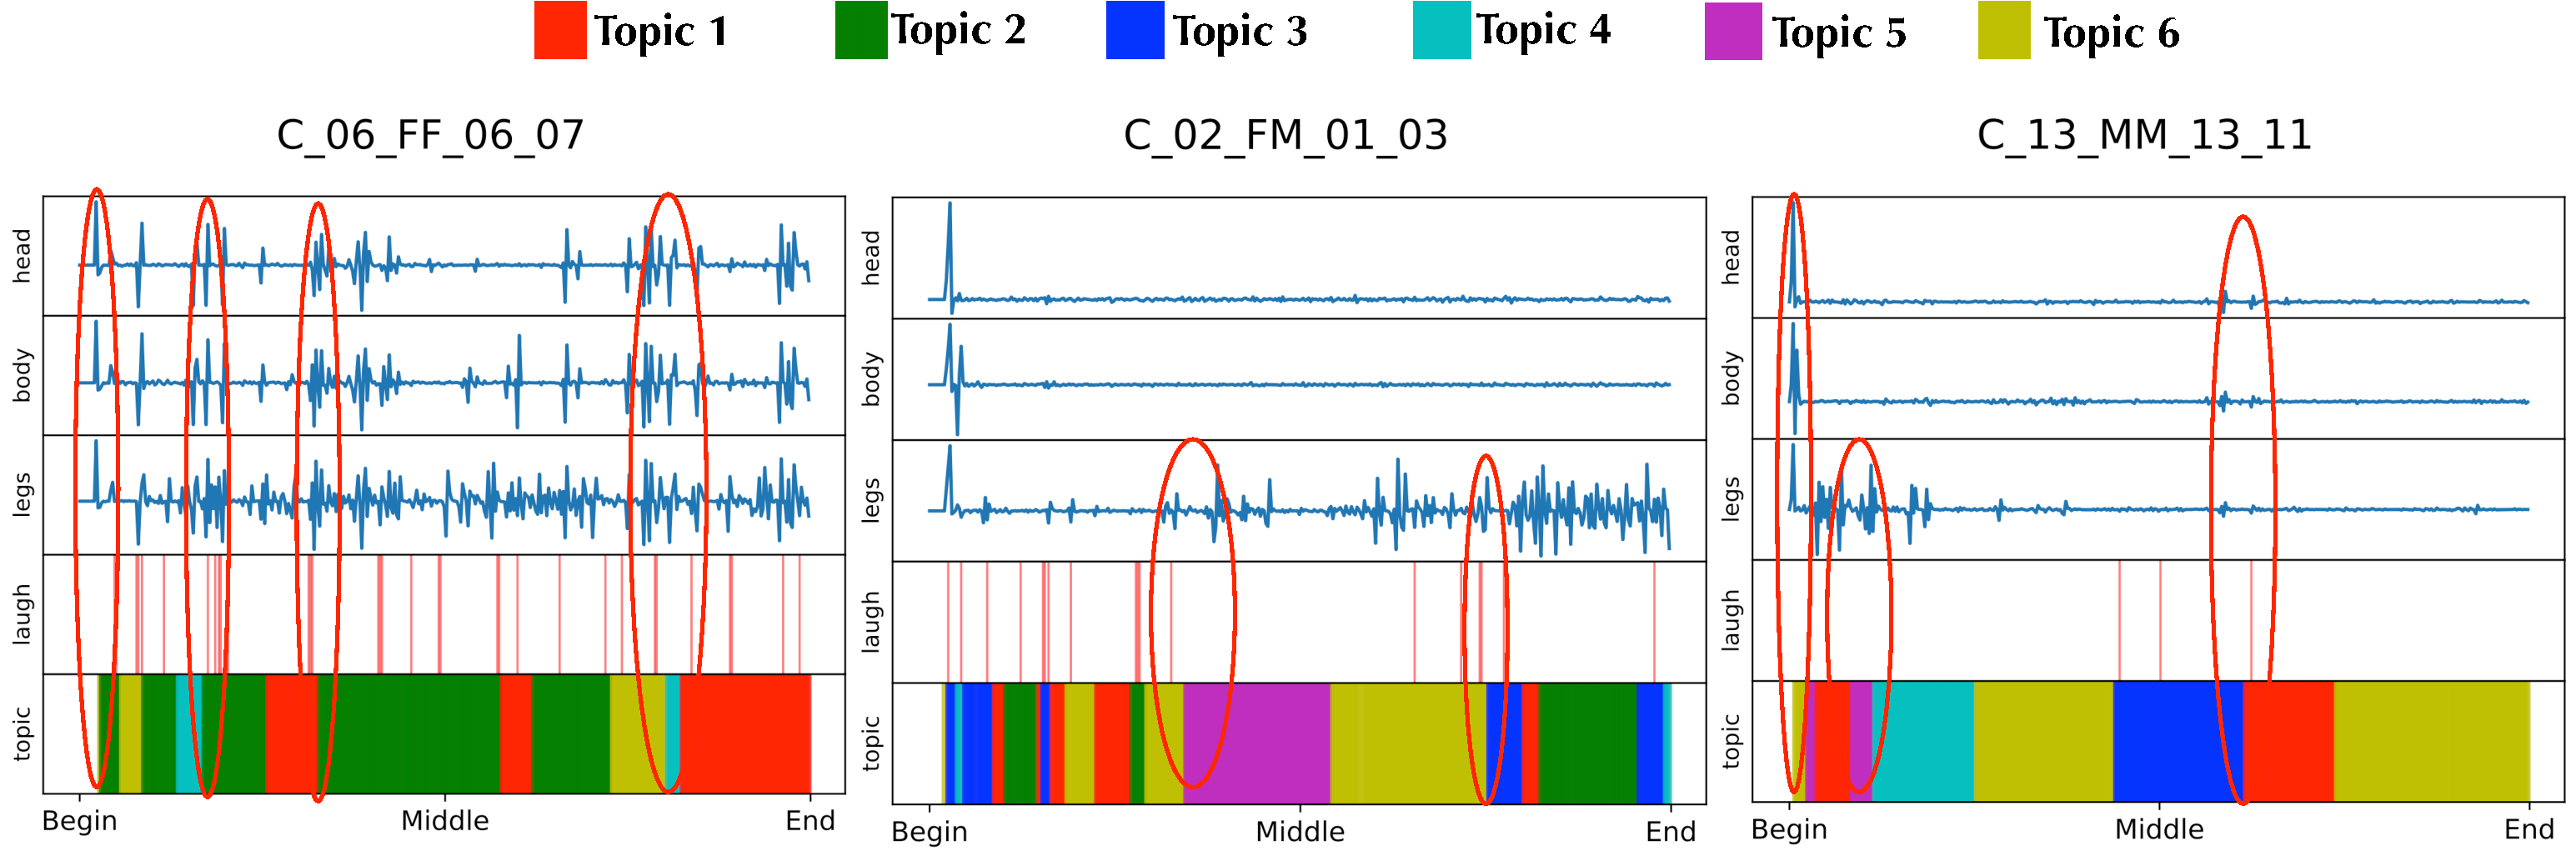
\includegraphics[width=\linewidth]{figures/multimodal.pdf}
  \caption{Time synchronized multi-modal features with topics, the fluctuation of the top three figure represents the intensity of both speakers movement in given body part. Three conversation between FF - two females, FM - female and male, MM - two male are selected in order from left to right. The topics are the same as from LDA model in Figure~\ref{fig:lda_topic}.}
  \label{fig:multimodal}
\end{figure*}

%%%%%%%%%%%%%%%%%%%%%%%%%%%%%%%%%%%%%%%%%%%%%%%%%%%%%%%%%%%%%%%%%%%%%%
%%% Section 8
\section{Automatic laughter detection}
\label{sec:automatic-laughter-detection}


\subsection{Acoustic system visualisation}
\label{sec:acoustic-visualisation}

Note that the acoustic features is highly non-linear, contradictory, LDA and PCA is linear dimension reduction method. Hence, the new projected space probably cannot capture all the discriminative properties between laugh and non-laugh signals.

Figures~\ref{fig:DS-pca-mfcc} and~\ref{fig:EE-pca-mfcc} illustrate the important of context window length in discriminating between laugh and non-laugh signals, as well as the differences between the DigiSami and Estonian corpora. Each MFCC features are processed using a window of 25 ms on input audio, and we shift the  window every 10 ms for the next features. We can see that there are significant amounts of laugh events which are longer than 0.25 ms, hence, 1 window of MFCC might not be enough to capture all necessary information that characterises the laughing. As a result, we group multiple windows and stack them into 1 big feature, the number of surrounding windows are called ``context windows''. For a context length equal to 10, it means we use 5 context windows in the past, and 5 context windows in the future to create a ``super vector'' feature. Figures~\ref{fig:DS-pca-mfcc} and~\ref{fig:EE-pca-mfcc} highlight the roles of context in laugh signal recognition. We can see that the longer the context the further the non-laugh (red) and laugh (blue) events are pushed into 2 sides of the figure, which is especially applied for Estonian dataset. On the other hand, the acoustic features of laugh signals in the DigiSami dataset are more difficult to separate from non-laugh signals compared to the Estonian dataset.

\begin{figure}[!t]
\centering
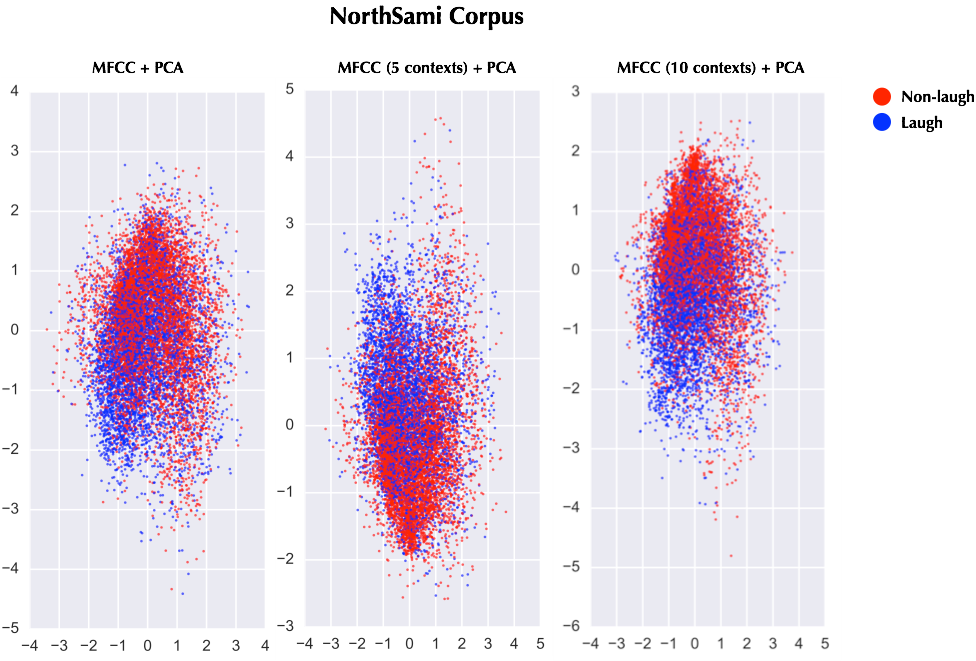
\includegraphics[width=1\linewidth]{images/PCA-MFCC-DS.png}
\caption{Applying Principal Components Analysis (PCA) on MFCC features with different amount of context windows for DigiSami Corpus.}
\label{fig:DS-pca-mfcc}
\end{figure}

\begin{figure}[!t]
\centering
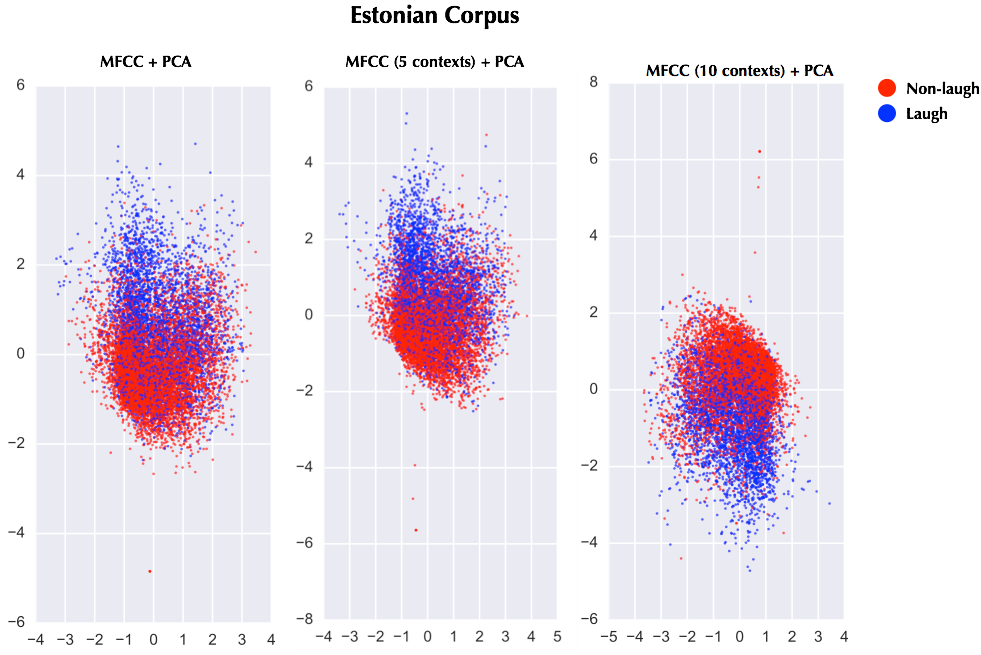
\includegraphics[width=1\linewidth]{images/PCA-MFCC-EE.png}
\caption{Applying Principal Components Analysis (PCA) on MFCC features with different amount of context windows for Estonian Corpus.}
\label{fig:EE-pca-mfcc}
\end{figure}


Figure~\ref{fig:applying-pca-and-lda} illustrates the effect of 2 algorithms on different features. We can see that non-laugh and laugh signals are more clearly separated in the case of MFCC with PCA. Using pitch features introduces more confusion between 2 kinds of data. However, both of them are clearly separated using LDA, hence, MFCC and pitch can probably used for training a classification between laugh and non-laugh events.

\begin{figure}[!t]
\centering
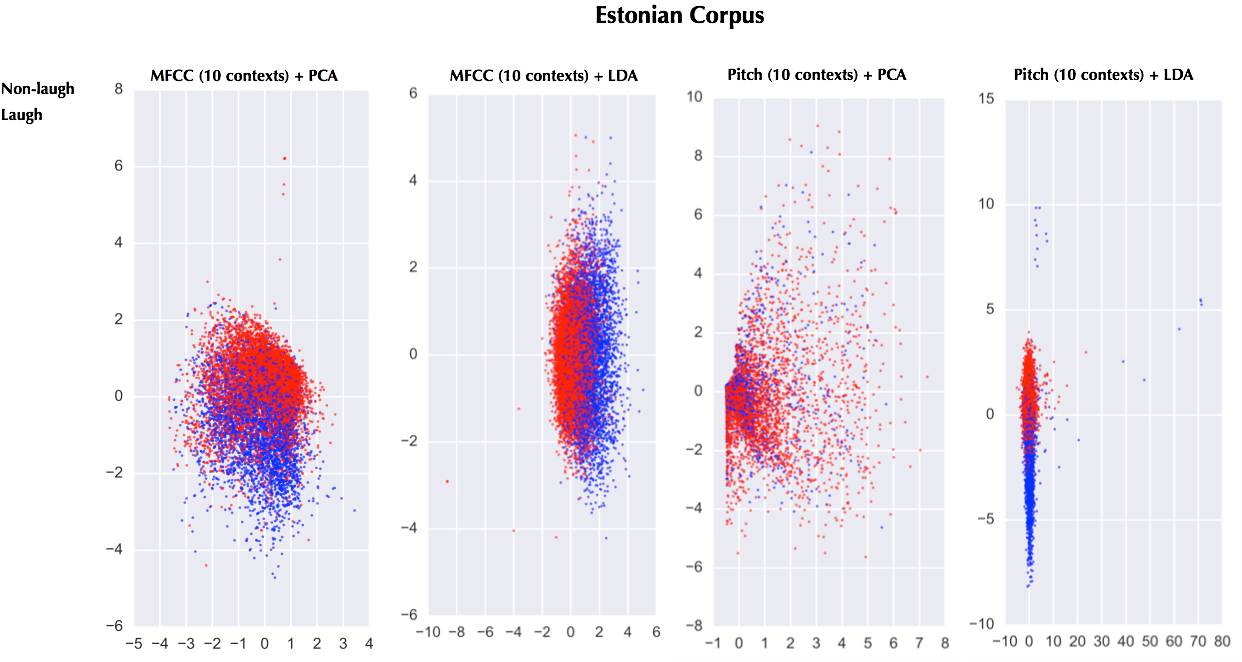
\includegraphics[width=1\linewidth]{images/ApplyingPCAandLDA-2.png}
\caption{Applying PCA and LDA on MFCC and PITCH as features.}
\label{fig:applying-pca-and-lda}
\end{figure}

Figure~\ref{fig:DS-pca-mfcc}, Figure~\ref{fig:EE-pca-mfcc} and Figure~\ref{fig:applying-pca-and-lda} emphasise the importance of features in detecting laugh events from audio signals.
We further investigate the influence these features on different types of laugh and dataset which is illustrated in
Figures~\ref{fig:lda-mfcc-laugh-types} and~\ref{fig:lda-mfcc-emotional-states}.

\begin{figure}[!t]
\centering
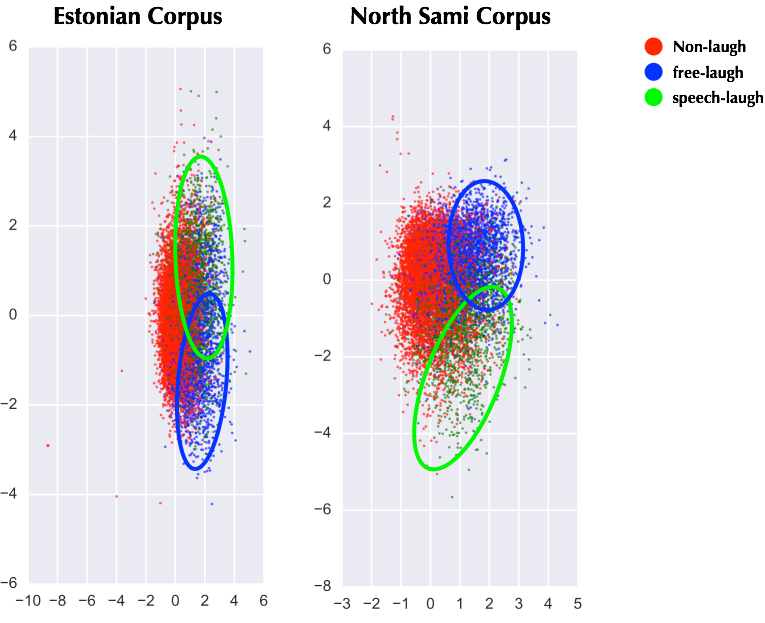
\includegraphics[width=1\linewidth]{images/LDA-MFCC-laugh-types.png}
\caption{Applying LDA on MFCC features with context windows of 10 for both dataset, with marked laugh types.}
\label{fig:lda-mfcc-laugh-types}
\end{figure}

In Figure~\ref{fig:lda-mfcc-laugh-types}, speech-laugh is clearly separated from free-laugh using LDA for 13 different laugh annotations (i.e. the labels are mixed of laugh types and emotional states). As a result, we can see that the laugh types are seemingly inferred given the mixed information of laugh and emotional states.

\begin{figure}[!t]
\centering
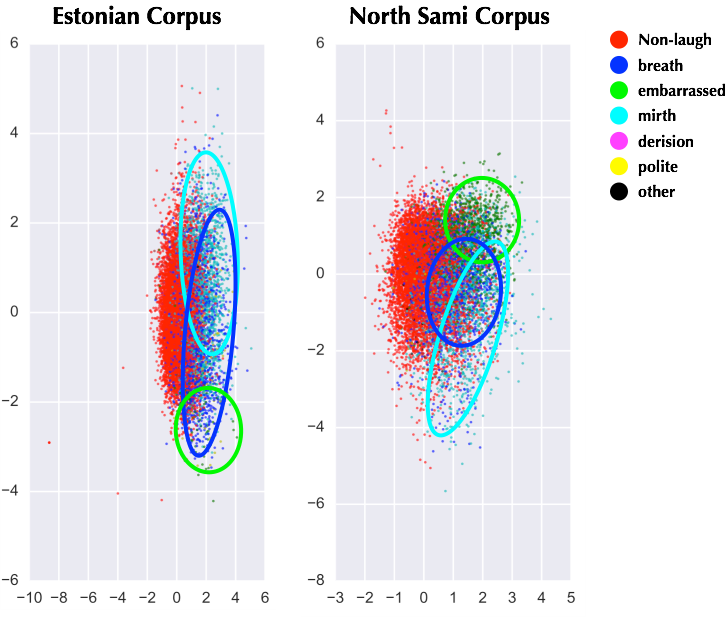
\includegraphics[width=1\linewidth]{images/LDA-MFCC-emotional-states.png}
\caption{Applying LDA on MFCC features with context windows of 10 for both dataset, with marked emotional states.}
\label{fig:lda-mfcc-emotional-states}
\end{figure}

However, Figure~\ref{fig:lda-mfcc-emotional-states} indicates the difficulty in extract emotional states information from all 13 annotations. We highlight the dense area of the three most popular states: breath, embarrassed and mirth. The circles are overlapped which illustrates strong confusion between different emotion

On the other hand, we can see the green zones of Figure~\ref{fig:lda-mfcc-laugh-types} match the mirth zones of Figure~\ref{fig:lda-mfcc-emotional-states}, hence, there exist strong relationship between speech-laugh events and mirth emotional state. Conversely, free-laugh is mixed of breath and embarrassed emotion, which make it more overlapped with non-laugh and speech-laugh signals.


\subsection{Acoustic system performance (binary classes)}
\label{sec:acoustic-performance-binary}

First, we treat the problem as laugh detection, where we try to recognise laugh event from audio signal. All of our experiments uses MFCC features, unless otherwise specified, all model use 24 context windows. For deep learning systems, a rectifier function is applied on each hidden layer and the output layer use sigmoid function. Moreover, convolution neural network has pooling layer with pool size of (2, 2) after each convolution with kernel size of (3, 3). Taking into account the fact that all results from our experiments are random variables, most of the experiments are run at least 3 times then we calculate the mean and standard deviation for each one. Table~\ref{tab:performance-binary} shows the performance of different algorithms on the binary classification task.

\begin{table*}[!t]
\caption{Performance of different algorithms on binary classification task.}
\label{tab:performance-binary}
\centering
%\begin{tabular}{| p{2.8cm} | p{1.1cm} | p{1.1cm}  | p{1.1cm}  | p{0.5cm}  |}
\begin{tabular}{| l | r | r  | r  | r |}
\hline
 & Accuracy & Precision & Recall & F1 \\
\hline
Logistic Regression & 95.5 & 0 & 0 & 0 \\
\hline
Linear SVM & $60.3 \pm 7.7$ & $4.3 \pm 0.5$ & $41.7 \pm 10.1$ & 8 \\
%Linear SVM & 60.3 & 4.3 & 41.7 & 8 \\
\hline
Deep learning (512-256) & $96.7 \pm 0.04$ & $79.0 \pm 2.2$ & $34.7 \pm 2.5$ & $48.0 \pm 2.2$ \\
%Deep learning & & & & \\
%(512-256) & 96.7 & 79.0 & 34.7 & 48.0 \\
\hline
Deep learning (512-256-128) & $96.8 \pm 0.1$ & $74.7 \pm 3.1$ & $40.3\pm 2.6$ & $52.3 \pm 1.9$ \\
%Deep learning & & & & \\
%(512-256-128) & 96.8 & 74.7 & 40.3 & 52.3 \\
\hline
Convolutional Neural Network & & & & \\
(32-64) & $96.8 \pm 0.05$ & $74.0 \pm 3.7$ & $41.3 \pm 4.5$ & $52.7 \pm 2.6$ \\
%Convolutional Neural Network & & & & \\
%(32-64) & 96.8 & 74.0 & 41.3 & 52.7 \\
\hline
Convolutional Neural Network & & & & \\
(32-64-64) context=80 & 97.1 & 76 & 47 & 58 \\
\hline
Convolutional Neural Network & & & & \\
(32-64-64) context=100 & 96.94 & 64 & 63 & 63 \\
\hline
Convolutional Neural Network & & & & \\
%(32-64-64) context=200 & 97.75 & 71.5 & 62.2 & 66.5 \\
(32-64-64) context=200 & $97.75 \pm 0.05$ & $71.5 \pm 2.5$ & $62.2 \pm 2.0$ & $66.5 \pm 0.5$ \\
\hline
Convolutional Neural Network & & & & \\
(32-64-64) context=250 & 97.6 & 60 & 73 & 66 \\
\hline

\end{tabular}
\end{table*}

Since our dataset is biased, as only 5.5\% of data represent laugh events, accuracy is an unreliable performance estimation. Precision represent positive predictive value: if our system is able to achieve 70\% of precision, it means that when we predict an audio segment is a laughing signal, we have 70\% chance to make the right prediction. On the other hand, detection rate (recall) is the amount of laugh events our system successfully detected (i.e. fraction of true laughing events that are retrieved). F1 score is the most reliable evaluation metric, since it balances the precision and detection rate and is not affected by a biased dataset.

From Table~\ref{tab:performance-binary}, we can see that Logistic Regression and Linear SVM are strongly biased toward non-laughing examples, both systems significantly misclassify non-laugh signals as laugh signals which resulted in high detection rate but very low precision. The deep learning systems are gradually improved by increasing the number of layers, but our further experiments indicated that 3 layers is the optimal number of layers for the given size of our dataset. By introducing convolutional neural networks, we were able to slightly raise the performance by 0.4\% (F1 score). Additionally, increasing the number of context windows from 24 to 200 significantly improves the overall performance, our best system achieves 71.5\% of precision with 62.2\% detection rate and F1 equal to 66.5\%. Since higher context length does not show improvement and requires more computational resource, 200 context windows are the optimal choice for the task.

Figure~\ref{fig:confusion-matrix-binary} shows the detailed performance of the best model. Since the model is better at detection, it makes less mistakes in mis-classifying non-laugh signals as laugh signals. However, there are many laughing samples that were ignored by the model, which is illustrated by the bottom left corner of the figure.

\begin{figure}[htb]
\centering
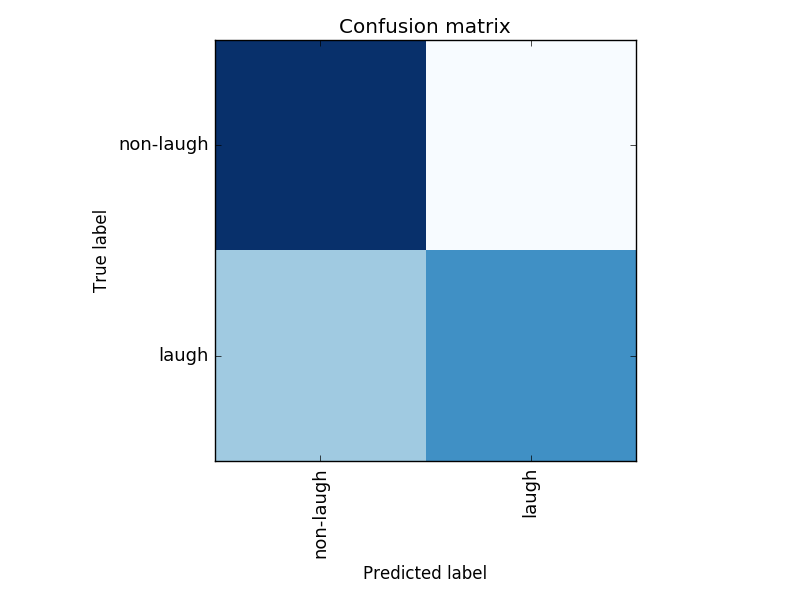
\includegraphics[width=1\linewidth]{images/ConfusionMatrix-Binary.png}
\caption{Confusion matrix on test data of the best model on binary classification task.}
\label{fig:confusion-matrix-binary}
\end{figure}


\subsection{Acoustic system performance (multiple classes)}
\label{sec:acoustic-performance-multi}

In the multi-classes classification task, we train a convolutional neural network to discriminate a mixed set of labels between laugh and emotional states (i.e. "fl, p" for free-laughter with polite intention).  The performance of the best algorithm is shown in Table~\ref{tab:performance-multi}, which is competitive to the best model in Section~\ref{sec:acoustic-performance-binary}.

\begin{table}[htb]
\caption{Performance of best algorithm on multi-class classification task.}
\label{tab:performance-multi}
\centering
\begin{tabular}{| p{2.8cm} | p{1.1cm} | p{1.1cm}  | p{1.1cm}  | p{0.5cm}  |}
\hline
 & Accuracy & Precision & Recall & F1 \\
\hline
Convolutional & & & & \\
Neural Network & & & & \\
(32-64-64) context=200 & 97.5 & 62.8 & 62.7 & 96.0 \\
\hline
\end{tabular}
\end{table}

Since the model simply ignores laughter types with smaller amounts of data and focusses on recognition of the ones with larger amounts of data, the confusion matrix in Figure~\ref{fig:confusion-matrix-multi} is biased. As ``fl, m'', ``st, m'', ``fl, b'' and ``st, e'' acquire about 95\% of laugh events, their performances are higher than other classes, and the system rarely misclassified their laugh signals as non-laugh signals.

\begin{figure}[htb]
\centering
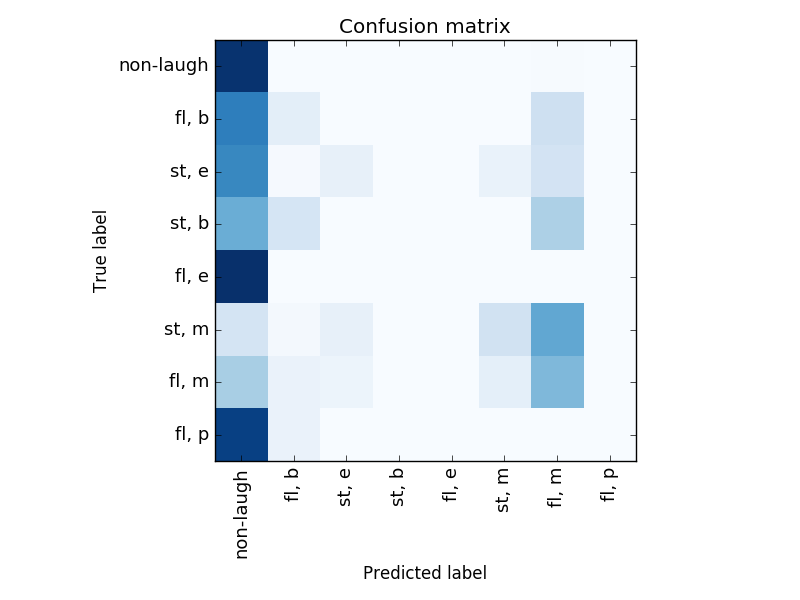
\includegraphics[width=1\linewidth]{images/ConfusionMatrix-Multi.png}
\caption{Confusion matrix on test data of the best model on multi-class classification task.}
\label{fig:confusion-matrix-multi}
\end{figure}

In conclusion, the binary classification task with a convolutional neural network achieves more stable results on the extremely skewed dataset, with good performance on both detection and precision.


\section{Discussion and Future Work}
\label{sec:discussion}

Our hypothesis concerning the acoustic differences of different laughter types was supported. In the DigiSami data,  durations of embarrassed laughs were significantly longer than the durations of all other types for both male and female informants, but we did not get support for the finding of Nwokah et al. \cite{Nwokah:ea:99} that speech-laughs are longer than free-laugh. As for the distinctions in intensity, this was small between the laugh types, but interestingly the women had higher intensity laughs than the men in our data.

The Estonian data had different laughter types compared to the DigiSami data: it had less embarrassed laughter, but a remarkable amount of polite laughter. In general, breathy and mirthful laughter were the majority of all laughter bouts. We hypothesize that the differences in the laughter types occur mainly because of very different relationship between the participants (first encounters in Esonian vs. mutually acquainted in DigiSami) and of the age of the participants (all adult in Estonian vs. partly high school students in DigiSami).

The comparison of acoustic analyses of our datasets showed the most remarkable differences in durational features of the different laughter types:  The Estonian data had the longest laughter bouts in mirthful types, while the polite and breathy types were the shortest. Both in the Estonian and DigiSami data, the embarrassed speech-laugh was the longest produced by both female and male participants. Interestingly, the longest laughter bout in the Estonian data was only 1.3 seconds, while in the DigiSami data the longest was 3.2 seconds, which is over twice as long as in the Estonian data.

The other two acoustic features, the F0 and intensity, showed no remarkable differences. In the DigiSami data it was clear that the F0 in free-laughter types was higher than F0 in speech-laughter for both male and female informants, which accords e.g. with Truong and van Leeuwen (2007), while in the Estonian data the polite free-laugh had the highest pitch of all laughter types, both for female and male participants.

In both datasets the intensity of different laughter types was rather similar, but the most surprising difference in the DigiSami data was that the average intensity with female informants was generally bigger than with males, while in the Estonian data many laughter types had higher intensity with male informants.

These observations will be substantiated with deeper statistical analysis, and models for joking, laughing and generally positive attitude will be explored further so as to enable appropriate models be implemented in the SamiTalk application \cite{Wilcock:ea:IWSDS:16}. A useful case is e.g. to be able to recognize the user's embarrassment or uncertainty on the basis of the amount of laughter and their role in the conversation, and alleviate such situations appropriately.

Moreover, as the collected data is multimodal, it is possible to study non-verbal as well as verbal communication. As argued in the previous research, the participants' engagement in the conversation and mutual bonding can be measured with the help of multimodal and non-verbal cues, such as the number of laughs or chuckles, or overlapping speech \cite{Bonin:16}. Our future studies concern the use of non-verbal information when laughing, to measure the participants' engagement in the interaction.


\section{Conclusion}
\label{sec:conclusion}

In this paper we have studied the interlocutors' laughing in the North Sami and Estonian interactions and the functions of laughter in conversational engagement. We can conclude that laughter has several functions that range from fun and happiness to a relief burst of embarrassment. We observed that laughter types depend on the situation and the role of the speakers, and we hypothesize that in natural conversations, the basic laughter types occur when the participants have real fun (mirth) or when they give breathy feedback (breath). However, if the situation is embarrassing or uncomfortable to the speaker, this is signalled by two extremes of laughter frequency, which differ depending on the participants' power relation: the peers use excessive laughter so as to share the embarrassing situation with the others, whereas the partners in an asymmetrical relation indicate more formal, non-sharing behaviour by the lack of laughter.



% use section* for acknowledgment
\ifCLASSOPTIONcompsoc
  % The Computer Society usually uses the plural form
  \section*{Acknowledgments}
\else
  % regular IEEE prefers the singular form
  \section*{Acknowledgment}
\fi

The authors gratefully acknowledge the Estonian and North Sami participants in the video recordings. The Estonian data was collected, transcribed, and annotated with the Estonian Science Foundation Project MINT (Multimododal Interaction, grant ETF8958).

The work has been conducted within the Academy of Finland project Finno-Ugric Digital Citizens
(grant n\textdegree270082).

The authors are also grateful to Dr Kevin El Haddad, Emer Gilmartin, and Khiet Truong for fruitful discussions.

% Can use something like this to put references on a page
% by themselves when using endfloat and the captionsoff option.
\ifCLASSOPTIONcaptionsoff
  \newpage
\fi



% trigger a \newpage just before the given reference
% number - used to balance the columns on the last page
% adjust value as needed - may need to be readjusted if
% the document is modified later
%\IEEEtriggeratref{8}
% The "triggered" command can be changed if desired:
%\IEEEtriggercmd{\enlargethispage{-5in}}

% references section

% can use a bibliography generated by BibTeX as a .bbl file
% BibTeX documentation can be easily obtained at:
% http://mirror.ctan.org/biblio/bibtex/contrib/doc/
% The IEEEtran BibTeX style support page is at:
% http://www.michaelshell.org/tex/ieeetran/bibtex/
\bibliographystyle{IEEEtran}
% argument is your BibTeX string definitions and bibliography database(s)
%\bibliography{IEEEabrv,../bib/paper}
\bibliography{../digisami}
%

% biography section
%
% If you have an EPS/PDF photo (graphicx package needed) extra braces are
% needed around the contents of the optional argument to biography to prevent
% the LaTeX parser from getting confused when it sees the complicated
% \includegraphics command within an optional argument. (You could create
% your own custom macro containing the \includegraphics command to make things
% simpler here.)
%\begin{IEEEbiography}[{\includegraphics[width=1in,height=1.25in,clip,keepaspectratio]{mshell}}]{Michael Shell}
% or if you just want to reserve a space for a photo:

\begin{IEEEbiography}{Kristiina Jokinen}
Biography text here.
\end{IEEEbiography}

% if you will not have a photo at all:
\begin{IEEEbiographynophoto}{John Doe}
Biography text here.
\end{IEEEbiographynophoto}

% insert where needed to balance the two columns on the last page with
% biographies
%\newpage

\begin{IEEEbiographynophoto}{Jane Doe}
Biography text here.
\end{IEEEbiographynophoto}

% You can push biographies down or up by placing
% a \vfill before or after them. The appropriate
% use of \vfill depends on what kind of text is
% on the last page and whether or not the columns
% are being equalized.

%\vfill

% Can be used to pull up biographies so that the bottom of the last one
% is flush with the other column.
%\enlargethispage{-5in}



% that's all folks
\end{document}


